% Biên dịch: xelatex main.tex (chạy 2 lần để có mục lục), hoặc dùng Overleaf với XeLaTeX.
\documentclass[12pt,a4paper]{report}

\usepackage{fontspec}
\setmainfont{TeX Gyre Termes}
\setmonofont{TeX Gyre Cursor}[Scale=0.88]
\usepackage[vietnamese]{babel}
\usepackage[a4paper,left=3cm,right=2cm,top=2.5cm,bottom=2.5cm]{geometry}
\usepackage{graphicx,booktabs,array,tabularx,longtable,xcolor,amsmath,enumitem,float,fancyhdr,setspace}
\usepackage{titlesec,tocloft,caption,listings,fvextra,tikz}
\usetikzlibrary{positioning,arrows.meta,shapes.geometric,fit,calc}
\usepackage{xurl}
\usepackage[hidelinks]{hyperref}
\urlstyle{tt}

\setstretch{1.15}
\setlength{\parskip}{3pt}
\setlength{\parindent}{1.2em}
\sloppy

% ----- Tiêu đề -----
\titleformat{\chapter}[block]{\centering\bfseries\Large}{CHƯƠNG \thechapter.}{0.5em}{}
\titlespacing*{\chapter}{0pt}{0pt}{18pt}
\titleformat{\section}{\bfseries\large}{\thesection.}{0.5em}{}
\titleformat{\subsection}{\bfseries\itshape}{\thesubsection.}{0.5em}{}
\renewcommand{\cftchappresnum}{CHƯƠNG }
\renewcommand{\cftchapaftersnum}{.}
\setlength{\cftchapnumwidth}{6.5em}
\renewcommand{\cftchapfont}{\bfseries}
\renewcommand{\cftchappagefont}{\bfseries}
\renewcommand{\contentsname}{Mục lục}
\renewcommand{\listfigurename}{Danh sách hình vẽ}
\renewcommand{\listtablename}{Danh sách bảng}
\renewcommand{\bibname}{TÀI LIỆU THAM KHẢO}
\captionsetup{font=small,labelfont=bf,labelsep=period}
\captionsetup[table]{position=top}
\renewcommand{\arraystretch}{1.15}
\pagestyle{fancy}\fancyhf{}\fancyfoot[C]{\thepage}\renewcommand{\headrulewidth}{0pt}
\fancypagestyle{plain}{\fancyhf{}\fancyfoot[C]{\thepage}\renewcommand{\headrulewidth}{0pt}}

\newcommand{\code}[1]{{\small\path{#1}}}
\definecolor{codebg}{gray}{0.95}
\lstset{basicstyle=\ttfamily\footnotesize,backgroundcolor=\color{codebg},frame=none,breaklines=true,
  columns=fullflexible,keepspaces=true,showstringspaces=false,xleftmargin=4pt,xrightmargin=4pt,
  keywordstyle=\bfseries,commentstyle=\itshape\color{gray}}
\expandafter\def\csname cellsetup\endcsname{1}
\expandafter\def\csname cellsplit\endcsname{2}
\expandafter\def\csname cellcompare\endcsname{3}
\expandafter\def\csname cellrocpr\endcsname{4}
\expandafter\def\csname cellcalib\endcsname{5}
\expandafter\def\csname cellbands\endcsname{6}
\expandafter\def\csname cellconfusion\endcsname{7}
\expandafter\def\csname cellkg\endcsname{8}
\expandafter\def\csname cellrl\endcsname{9}

\newcommand{\nbcell}[2]{\par\medskip\noindent\textbf{Cell~\csname cell#1\endcsname{} của \texttt{training.ipynb}}: #2\par\smallskip\VerbatimInput[fontsize=\scriptsize,frame=leftline,rulecolor=\color{gray},framesep=4pt,breaklines=true,breakanywhere=true]{cells/#1.py}\par\medskip}
\newcolumntype{L}[1]{>{\raggedright\arraybackslash}p{#1}}

\begin{document}

% ================= TRANG BÌA =================
\begin{titlepage}
\thispagestyle{empty}
\begin{tikzpicture}[remember picture,overlay]
  \draw[line width=1.2pt] ([shift={(2.3cm,-1.5cm)}]current page.north west) rectangle ([shift={(-1.5cm,1.5cm)}]current page.south east);
  \draw[line width=0.4pt] ([shift={(2.45cm,-1.65cm)}]current page.north west) rectangle ([shift={(-1.65cm,1.65cm)}]current page.south east);
\end{tikzpicture}
\begin{center}
\vspace*{0.8cm}
{\bfseries HỌC VIỆN CÔNG NGHỆ BƯU CHÍNH VIỄN THÔNG}\\[0.5cm]
{\bfseries KHOA CÔNG NGHỆ THÔNG TIN 1}\\[-0.1cm]
\rule{5cm}{0.4pt}\\[3.2cm]
{\bfseries\Huge PROJECT 01}\\[0.4cm]
{\bfseries\LARGE PHÁT TRIỂN HỆ THỐNG THÔNG MINH}\\[1.6cm]
{\bfseries\Large HỆ ĐA AGENT HỖ TRỢ SÀNG LỌC\\NGUY CƠ BỆNH TIỂU ĐƯỜNG}\\[0.5cm]
{\itshape Deep Learning, Knowledge Base (Neo4j) và RAG,\\Reinforcement Learning kết hợp luật}\\[3.3cm]
\begin{tabular}{@{}l@{\hspace{1.2em}}l@{}}
\bfseries Giảng viên hướng dẫn: & PGS. TS. Trần Đình Quế\\[3pt]
\bfseries Sinh viên thực hiện: & Trần Hải Long\\[3pt]
\bfseries Mã sinh viên: & B23DCCN510\\[3pt]
\bfseries Nhóm lớp: & 06\\[3pt]
\bfseries Nhóm: & 03
\end{tabular}
\vfill
{\bfseries Hà Nội, tháng 11 năm 2026}\\[0.8cm]
\end{center}
\end{titlepage}

\pagenumbering{roman}
\setcounter{page}{2}
\tableofcontents
\clearpage

% ================= TỪ VIẾT TẮT =================
\chapter*{DANH MỤC TỪ VIẾT TẮT}
\addcontentsline{toc}{chapter}{DANH MỤC TỪ VIẾT TẮT}
\begin{center}
\begin{tabular}{@{}L{2.2cm}L{5.2cm}L{5.8cm}@{}}
\toprule
\textbf{Viết tắt} & \textbf{Tiếng Anh} & \textbf{Tiếng Việt}\\
\midrule
ADA & American Diabetes Association & Hiệp hội Đái tháo đường Hoa Kỳ\\
AP & Average Precision & Độ chính xác trung bình (diện tích dưới đường PR)\\
AUC & Area Under the (ROC) Curve & Diện tích dưới đường ROC\\
BMI & Body Mass Index & Chỉ số khối cơ thể\\
BRFSS & Behavioral Risk Factor Surveillance System & Hệ thống giám sát yếu tố nguy cơ hành vi (CDC)\\
CV & Cross-Validation & Kiểm chứng chéo\\
DL & Deep Learning & Học sâu\\
ĐTĐ & -- & Đái tháo đường\\
FPG & Fasting Plasma Glucose & Glucose huyết tương lúc đói\\
HbA1c (A1C) & Glycated Hemoglobin & Huyết sắc tố gắn glucose\\
HNSW & Hierarchical Navigable Small World & Đồ thị thế giới nhỏ phân cấp\\
KB & Knowledge Base & Cơ sở tri thức\\
LLM & Large Language Model & Mô hình ngôn ngữ lớn\\
MAS & Multi-Agent System & Hệ đa tác tử (hệ đa agent)\\
MDP & Markov Decision Process & Quá trình quyết định Markov\\
ML & Machine Learning & Học máy\\
MLP & Multilayer Perceptron & Mạng nơ-ron nhiều lớp\\
RAG & Retrieval-Augmented Generation & Sinh văn bản tăng cường truy xuất\\
RL & Reinforcement Learning & Học tăng cường\\
ROC & Receiver Operating Characteristic & Đường đặc trưng hoạt động của bộ thu\\
\bottomrule
\end{tabular}
\end{center}
\clearpage

\listoffigures
\clearpage
\listoftables
\clearpage

\pagenumbering{arabic}
\setcounter{page}{1}

% ================= CHƯƠNG 1 =================
\chapter{GIỚI THIỆU}

\section{Bài toán và động lực}
Đái tháo đường (ĐTĐ, bệnh tiểu đường) là tình trạng glucose trong máu tăng cao kéo dài do cơ thể thiếu insulin hoặc kháng insulin. Phần lớn ca bệnh là ĐTĐ típ 2, tiến triển âm thầm nhiều năm và có thể được làm chậm hoặc phòng ngừa nếu phát hiện sớm từ giai đoạn tiền ĐTĐ \cite{ada2025,dpp2002}. Người dân thường chỉ có vài con số rời rạc (một lần thử đường huyết, cân nặng, huyết áp) và không biết chúng nói lên điều gì.

Một công cụ hỗ trợ sàng lọc cần làm được bốn việc: \emph{dự đoán} nguy cơ từ dữ liệu sức khỏe; \emph{giải thích} dựa trên tri thức y khoa có nguồn; \emph{gợi ý} bước tiếp theo; và \emph{cảnh báo} khi số đo ở mức nguy hiểm. Mỗi việc cần một kỹ thuật khác nhau: học sâu cho dự đoán, cơ sở tri thức và RAG cho giải thích, học tăng cường cho việc chọn bước hỗ trợ, và luật tường minh cho an toàn. Gộp tất cả vào một chương trình làm hệ thống khó kiểm thử và khó tin cậy. Vì vậy dự án tách thành các thành phần chuyên trách, do một Orchestrator điều phối.

\section{Mục tiêu và phạm vi}
Dự án hiện thực hóa sơ đồ do giảng viên đưa ra trên lớp (Hình~\ref{fig:arch}, Chương~3) thành một hệ thống chạy được đầu--cuối:
\begin{itemize}[nosep]
\item \textbf{DB $\rightarrow$ Deep Learning $\rightarrow$ dự đoán, phân loại}: huấn luyện và so sánh năm mô hình học máy/học sâu trên bộ dữ liệu CDC Diabetes Health Indicators (BRFSS 2015, 253.680 hồ sơ, 21 đặc trưng); chọn mạng MLP (PyTorch) đã hiệu chuẩn xác suất; phân tầng nguy cơ thành ba mức Thấp, Trung bình, Cao.
\item \textbf{Web, sách $\rightarrow$ Neo4j KB $\rightarrow$ RAG}: đồ thị tri thức về ĐTĐ (20 thực thể, 35 quan hệ, 21 đoạn bằng chứng từ 5 nguồn) trên Neo4j; các đoạn bằng chứng được nhúng bằng \code{all-MiniLM-L6-v2} và tìm kiếm theo độ tương đồng trên ChromaDB, kết hợp với liên kết từ đồ thị.
\item \textbf{Reinforcement learning + rule $\rightarrow$ Agent}: chính sách Q-learning chọn bước hỗ trợ tiếp theo, luôn nằm dưới quyền ưu tiên của bộ luật an toàn.
\item \textbf{Tư vấn, trợ giúp}: giải thích đặc trưng, khuyến nghị có trích dẫn nguồn, câu hỏi bổ sung theo mức ảnh hưởng và mô phỏng \emph{``nếu thay đổi''}.
\item \textbf{Code + Demo}: API FastAPI, giao diện web Next.js, bộ kiểm thử tự động.
\end{itemize}
\textbf{Phạm vi.} Đây là sản phẩm học tập. Hệ thống phục vụ \emph{sàng lọc} chứ không \emph{chẩn đoán}, không đưa liều thuốc, và mọi kết quả đều nhắc người dùng đi khám bác sĩ. Các con số trong báo cáo được lấy từ \code{artifacts/}, từ lần chạy kiểm thử và từ ví dụ chạy trực tiếp trên mã nguồn của dự án; các giả định chưa kiểm chứng được nêu rõ.

\section{Đóng góp và cấu trúc báo cáo}
Các đóng góp chính:
\begin{itemize}[nosep]
\item Quy trình huấn luyện có kỷ luật đánh giá: chia 60/20/20 có phân tầng, CV 5 lần, tuning hai mô hình đứng đầu, chọn mô hình và ngưỡng \emph{trên tập kiểm định}, chỉ dùng tập kiểm tra để đánh giá cuối.
\item Tách ngưỡng nhị phân và các mức Thấp/Trung bình/Cao nhưng cùng chọn trên kiểm định, để một ca bị gắn cờ dương tính không bao giờ ở mức Thấp.
\item Bộ luật an toàn có mã luật, mức ưu tiên và căn cứ; \emph{số đo thực tế thắng dự đoán thống kê}, và mọi xung đột được báo cáo cùng cách giải quyết.
\item Truy xuất bằng chứng từ đồ thị tri thức Neo4j kết hợp tìm kiếm ngữ nghĩa, mỗi khẳng định trích dẫn được tới nguồn.
\item Policy Q-learning chọn bước hỗ trợ tiếp theo, so sánh với các chiến lược cố định, và ghi rõ phản hồi là \emph{mô phỏng}.
\item Cô lập lỗi: lỗi của thành phần tùy chọn được ghi vào \code{degraded}, có nội dung dự phòng; lỗi bộ luật nghiêng về phía chuyển bác sĩ.
\end{itemize}
Báo cáo gồm: Chương~2 cơ sở về agent và hệ đa agent; Chương~3 kiến trúc tổng quan; Chương~4 từng thành phần; Chương~5 mã nguồn, demo, kiểm thử và đánh giá; cuối cùng là kết luận.

% ================= CHƯƠNG 2 =================
\chapter{HỆ ĐA AGENT}

\section{Agent}
Theo Wooldridge \cite{wooldridge2009}, agent (tác tử) là một hệ thống tính toán đặt trong một môi trường, có khả năng \emph{hành động tự chủ} trong môi trường đó để đạt mục tiêu được giao. Điều cốt lõi là vòng lặp quan sát $\rightarrow$ quyết định $\rightarrow$ hành động $\rightarrow$ nhận phản hồi. Một agent thông minh có bốn tính chất \cite{jennings1998}: tự chủ, phản ứng, chủ động và xã hội.

Russell và Norvig \cite{russell2021} phân loại agent theo độ phức tạp của chương trình bên trong. Bảng~\ref{tab:agenttypes} đặt các thành phần của dự án vào cách phân loại đó. Cần lưu ý đây là phép ánh xạ tương đối: một số thành phần (như bộ luật) đơn giản hơn một agent đầy đủ và được gọi là ``thành phần'' thay vì ``agent''.

\begin{table}[H]
\centering
\caption{Các loại agent và hiện thực trong dự án}\label{tab:agenttypes}
\begin{tabularx}{\textwidth}{@{}L{3cm}L{3.8cm}X@{}}
\toprule
\textbf{Loại} & \textbf{Cách ra quyết định} & \textbf{Trong dự án}\\
\midrule
Phản xạ theo luật & Nếu điều kiện thì hành động; không học & \code{SafetyGuard} + \code{RuleEngine} (9 luật: 5 luật cơ sở, 4 luật xung đột)\\
Có trạng thái & Duy trì bộ nhớ & \code{MemoryAgent} lưu dự đoán trong ChromaDB và tìm hồ sơ tương tự\\
Dựa trên tri thức & Suy luận trên tri thức tường minh & \code{RetrievalAgent}: KB Neo4j + tìm kiếm ngữ nghĩa\\
Dựa trên mục tiêu (đơn giản) & Chọn chuỗi bước để đạt mục tiêu & \code{Orchestrator}: quy trình cố định; riêng việc ``thu thập thêm'' do policy chọn (tối đa 3 bước)\\
Agent học & Cải thiện từ dữ liệu, phần thưởng & \code{RiskModel} (MLP, học có giám sát); \code{QPolicy} (Q-learning)\\
Sinh văn bản & Diễn đạt kết quả của các thành phần khác & \code{ExplanationAgent}, \code{RecommendationAgent} (LLM tùy chọn; mặc định dùng mẫu câu)\\
\bottomrule
\end{tabularx}
\end{table}

\section{Hệ đa agent}
Hệ đa agent (Multi-Agent System, MAS) gồm nhiều agent tương tác để giải quyết bài toán vượt quá khả năng hoặc hiểu biết của từng agent. Nếu chỉ có một khối làm tất cả, nó phải trộn dữ liệu số, văn bản y khoa, chính sách chọn bước và luật an toàn trong cùng một chỗ: khó kiểm thử, khó thay thế và khó biết kết luận đến từ đâu. Bảng~\ref{tab:single-vs-multi} so sánh hai cách làm.

\begin{table}[H]
\centering
\caption{Một khối làm tất cả so với hệ nhiều thành phần của dự án}\label{tab:single-vs-multi}
\begin{tabularx}{\textwidth}{@{}L{3cm}L{4.5cm}X@{}}
\toprule
\textbf{Tiêu chí} & \textbf{Một khối} & \textbf{Nhiều thành phần (dự án)}\\
\midrule
Độ phức tạp & Cao, trộn nhiều kỹ thuật & Mỗi thành phần một kỹ thuật\\
Kiểm thử & Khó tách lỗi & Kiểm thử riêng từng thành phần (15 tệp kiểm thử)\\
An toàn & Luật nằm lẫn trong mô hình & Bộ luật độc lập, luôn ưu tiên hơn dự đoán và policy RL\\
Chịu lỗi & Một lỗi làm hỏng cả yêu cầu & Lỗi được ghi vào \code{degraded}, dùng nội dung dự phòng\\
Chi phí phối hợp & Không có & Cần Orchestrator và định dạng dữ liệu trao đổi thống nhất\\
\bottomrule
\end{tabularx}
\end{table}

\textbf{Mô hình tổ chức.} Dự án dùng kiểu \emph{supervisor}: Orchestrator gọi các thành phần theo thứ tự, truyền kết quả giữa chúng và tổng hợp đầu ra. Không có agent nào gọi trực tiếp agent khác.

\section{Giao tiếp giữa các thành phần}
FIPA-ACL \cite{fipa2002} chuẩn hóa thông điệp giữa các agent bằng \emph{performative}. Dự án \textbf{không} hiện thực đầy đủ FIPA-ACL và không có bus thông điệp bất đồng bộ. Giao tiếp gồm hai tầng:
\begin{itemize}[nosep]
\item \textbf{Dữ liệu có cấu trúc}: các thành phần được Orchestrator gọi như hàm Python và trao đổi từ điển JSON có trường rõ ràng, ví dụ \code{prediction}, \code{feature_explanation}, \code{retrieved_context}, \code{safety}, \code{policy}. Đủ cho một quy trình tuần tự và dễ kiểm thử.
\item \textbf{Thông điệp có kiểu khi các kết luận bất đồng}: một tập con nhỏ của FIPA-ACL (\code{agents/dialogue.py}) gồm bốn performative \code{challenge}, \code{accept}, \code{propose}, \code{inform}. Khi một luật xung đột kích hoạt, \code{SafetyGuard} gửi \code{challenge} tới thành phần bị luật bác bỏ; thành phần đó trả lời bằng hàm phản hồi riêng của mình. Một loại đề xuất, \code{propose} kèm \code{action}, được Orchestrator thực hiện thật và kết quả được báo lại bằng \code{inform} (Mục~4.4).
\end{itemize}

Để vẫn truy vết được ``ai đã làm gì'', lớp \code{RunLog} ghi lại mỗi bước (tên thành phần, trạng thái \code{ok}/\code{degraded}, thời gian xử lý bằng mili-giây, mô tả ngắn). Trường \code{trace} trong kết quả API chứa toàn bộ các bước này, cùng danh sách thông điệp \code{trace.dialogue} giữa các thành phần, và được giao diện hiển thị ở mục ``Cả đội đã làm việc thế nào''.

\textbf{Hướng lai LLM.} Các mô hình ngôn ngữ lớn thường được dùng làm ``bộ não'' của agent, kéo theo rủi ro ảo giác lan truyền và chi phí gọi nhiều lần. Dự án chọn hướng lai: mọi quyết định lâm sàng do mô hình đã đánh giá và luật tường minh đảm nhận; LLM (OpenAI, mặc định \code{gpt-4o-mini}) chỉ \emph{diễn đạt} giải thích và khuyến nghị khi có \code{OPENAI_API_KEY}. Thiếu khóa hoặc gọi lỗi thì dùng mẫu câu dự phòng và nói rõ điều đó. Nhờ vậy toàn bộ hệ thống chạy được không cần LLM và cho kết quả tái lập.

% ================= CHƯƠNG 3 =================
\chapter{KIẾN TRÚC TỔNG QUAN}

\section{Sơ đồ của đề bài và hiện thực}
Hình~\ref{fig:arch} vẽ lại sơ đồ của đề bài kèm thành phần hiện thực. Có ba dòng chảy hội tụ vào Orchestrator: (1) dữ liệu có sẵn đi qua Deep Learning để dự đoán và phân loại; (2) tri thức từ các nguồn y khoa được tạo thành Knowledge Base trên Neo4j và truy xuất bằng RAG; (3) bộ luật và policy reinforcement learning cùng điều khiển việc ra quyết định. Kết quả hội tụ ở đầu ra tư vấn và trợ giúp có kèm bằng chứng.

\begin{figure}[H]
\centering
\resizebox{\textwidth}{!}{%
\begin{tikzpicture}[
  node distance=0.55cm and 0.9cm,
  box/.style={draw,rounded corners=2pt,align=center,minimum height=0.95cm,inner sep=4pt,font=\small},
  data/.style={draw,cylinder,shape border rotate=90,aspect=0.25,align=center,font=\small,minimum height=1.2cm},
  note/.style={font=\scriptsize\itshape,gray,align=center},
  arr/.style={-{Stealth[length=2.2mm]},thick}]
\node[data] (db) {Dữ liệu BRFSS 2015\\253.680 hồ sơ};
\node[box,right=of db] (dl) {Deep Learning\\MLP + 4 mô hình đối chứng};
\node[box,right=of dl] (pred) {Dự đoán, phân loại\\xác suất · Thấp/TB/Cao};
\node[data,below=1.6cm of db] (kb) {KB Neo4j\\20 thực thể · 35 quan hệ\\21 đoạn bằng chứng};
\node[box,right=of kb] (rag) {RAG\\MiniLM + ChromaDB\\+ liên kết đồ thị};
\node[box,right=of rag] (ret) {RetrievalAgent};
\node[box,below=1.4cm of rag,fill=blue!6] (orch) {\textbf{Orchestrator}\\điều phối, tổng hợp, \code{trace}};
\node[box,left=of orch] (rule) {Bộ luật an toàn\\9 luật};
\node[box,right=of orch] (rl) {Policy Q-learning\\108 trạng thái · 5 hành động};
\node[box,below=1.3cm of orch,fill=green!6] (out) {Tư vấn và trợ giúp\\giải thích · khuyến nghị có trích dẫn · câu hỏi bổ sung · \emph{what-if}};
\draw[arr] (db)--(dl); \draw[arr] (dl)--(pred);
\draw[arr] (kb)--(rag); \draw[arr] (rag)--(ret);
\draw[arr] (pred.south) |- ([yshift=0.35cm]orch.north west) -- ([yshift=0.0cm,xshift=0.2cm]orch.north west);
\draw[arr] (ret.south) |- ([yshift=0.35cm]orch.north east) -- ([xshift=-0.2cm]orch.north east);
\draw[arr] (rule)--(orch); \draw[arr] (rl)--(orch);
\draw[arr] (orch)--(out);
\node[note,above=0.05cm of dl] {PyTorch · scikit-learn · LightGBM};
\node[note,below=0.05cm of rl] {phản hồi mô phỏng};
\end{tikzpicture}}
\caption{Sơ đồ hệ thống theo đề bài, kèm thành phần hiện thực của dự án}\label{fig:arch}
\end{figure}

Bảng~\ref{tab:map} ánh xạ từng khối trên sơ đồ sang mã nguồn.

\begin{table}[H]
\centering
\caption{Ánh xạ khối trên sơ đồ sang thành phần của hệ thống}\label{tab:map}
\begin{tabularx}{\textwidth}{@{}L{3.2cm}L{4.1cm}X@{}}
\toprule
\textbf{Khối trên sơ đồ} & \textbf{Thành phần} & \textbf{Hiện thực}\\
\midrule
DB $\rightarrow$ Deep learning $\rightarrow$ Dự đoán, Phân loại & \code{models/}, \code{RiskModel} & Huấn luyện bằng \code{training_pipeline.py}; MLP PyTorch, suy luận bằng NumPy; ngưỡng và mức nguy cơ lưu trong artifact (Mục~4.1)\\
Neo4j KB & \code{tools/neo4j_kb.py}, \code{scripts/collect_corpus.py} & Thu thập web/PDF, ghép đồ thị tuyển chọn trong bộ nhớ, kiểm tra rồi nạp (\code{MERGE}) trực tiếp vào Neo4j; ứng dụng bắt buộc dùng Neo4j (Mục~4.2)\\
RAG $\rightarrow$ Agent & \code{RetrievalAgent} & Nhúng \code{all-MiniLM-L6-v2}, chỉ mục ChromaDB (cosine), cộng điểm cho đoạn gắn với yếu tố nguy cơ qua đồ thị\\
Bộ luật & \code{SafetyGuard}, \code{RuleEngine} & 5 luật cơ sở và 4 luật xung đột (Mục~4.3)\\
Reinforcement learning & \code{rl/environment.py}, \code{rl/policy.py} & Q-learning dạng bảng trên môi trường mô phỏng (Mục~4.3)\\
Tư vấn, trợ giúp & \code{ExplanationAgent}, \code{RecommendationAgent}, \code{what_if}, \code{patient_guidance} & Giải thích, khuyến nghị có trích dẫn, mô phỏng ``nếu thay đổi'', câu hỏi bổ sung (Mục~4.4)\\
\bottomrule
\end{tabularx}
\end{table}

\section{Vai trò của các thành phần}
\begin{table}[H]
\centering
\caption{Các thành phần, đầu vào và kỹ thuật bên trong}\label{tab:components}
\begin{tabularx}{\textwidth}{@{}L{3.3cm}L{3.9cm}X@{}}
\toprule
\textbf{Thành phần} & \textbf{Nhận} & \textbf{Vai trò và kỹ thuật}\\
\midrule
\code{Orchestrator} & Hồ sơ đã kiểm tra từ API & Gọi lần lượt các thành phần, truyền kết quả, ghi \code{trace}, xử lý lỗi, thương lượng giữa các thành phần (\code{_negotiate}), chạy vòng policy (tối đa 3 bước)\\
\code{RiskModel} & Hồ sơ (tuổi, giới, chiều cao, cân nặng, huyết áp, các mục tùy chọn) & Chuẩn hóa về 21 đặc trưng BRFSS, dự đoán xác suất bằng MLP hiệu chuẩn, ghi nhận trường tự điền\\
\code{FeatureExplainer} & Hồ sơ & Giải thích bằng phân tích độ nhạy (SHAP chỉ cho mô hình tuyến tính)\\
\code{RetrievalAgent} & Hồ sơ, mức nguy cơ, giải thích đặc trưng & Tìm tối đa 3 đoạn bằng chứng (5 khi mở rộng), trả nguồn, URL, độ liên quan, \code{evidence_status}\\
\code{MemoryAgent} & Hồ sơ, xác suất & Lưu dự đoán; tìm hồ sơ tương tự theo khoảng cách số (tuổi, BMI, huyết áp, glucose)\\
\code{SafetyGuard} & Hồ sơ, xác suất, mức nguy cơ, trạng thái bằng chứng & Chạy bộ luật, tính điểm chất lượng dữ liệu, xác định mức chuyển tuyến\\
\code{QPolicy} & Trạng thái 5 chiều & Chọn bước tiếp theo từ bảng Q\\
\code{RecommendationAgent} & Bằng chứng, ca tương tự, kết quả luật, giải thích đặc trưng & Khuyến nghị có trích dẫn \code{[n]} (LLM tùy chọn; mẫu câu dự phòng)\\
\code{ExplanationAgent} & Kết quả cuối của các thành phần & Giải thích bằng lời, chạy sau cùng\\
\code{WhatIfSimulator} & Hồ sơ & Tính lại xác suất khi thay đổi một yếu tố có thể thay đổi\\
\bottomrule
\end{tabularx}
\end{table}

\section{Luồng một lượt đánh giá}
Mỗi yêu cầu \code{POST /v1/predict} đi qua các bước sau (Hình~\ref{fig:flow}); các bước tùy chọn được bọc bởi \code{RunLog.guard} nên lỗi của chúng không làm hỏng cả yêu cầu:
\begin{enumerate}[nosep]
\item API kiểm tra dữ liệu (cần BMI \emph{hoặc} đủ chiều cao và cân nặng, nếu không trả HTTP 422).
\item \code{RiskModel} dự đoán; xác định nhãn nhị phân và mức nguy cơ theo ngưỡng trong artifact.
\item Tính độ nhạy đặc trưng, tìm hồ sơ tương tự, truy xuất bằng chứng.
\item Đánh giá \code{evidence_status}, chạy bộ luật, soạn khuyến nghị.
\item \emph{Thương lượng}: nếu có luật xung đột, các thành phần trao đổi thông điệp (Mục~4.4); đề xuất ``tìm mở rộng bằng chứng'' của \code{RetrievalAgent} được thực hiện ngay (chạy lại truy xuất, luật và khuyến nghị), tối đa một lần.
\item Nếu có policy: dựng trạng thái (đã tính việc tìm mở rộng ở bước trước), hỏi policy; nếu chọn ``tìm thêm bằng chứng'' thì chạy lại truy xuất mở rộng, luật và khuyến nghị (tối đa 3 bước).
\item Mô phỏng ``nếu thay đổi'' (chỉ khi mức chuyển tuyến là theo dõi định kỳ), giải thích cuối, lưu bộ nhớ, ghi audit.
\end{enumerate}

\begin{figure}[H]
\centering
\begin{tikzpicture}[node distance=0.45cm,
  s/.style={draw,rounded corners=2pt,align=center,minimum width=3.6cm,minimum height=0.75cm,font=\small},
  r/.style={s,fill=red!6},g/.style={s,fill=green!6},b/.style={s,fill=blue!6},
  arr/.style={-{Stealth[length=2mm]},thick}]
\node[s] (a) {Hồ sơ từ giao diện / API (kiểm tra đầu vào)};
\node[b,below=of a] (b1) {\code{RiskModel}: xác suất, mức nguy cơ};
\node[b,below=of b1] (b2) {Giải thích đặc trưng · hồ sơ tương tự · truy xuất bằng chứng};
\node[r,below=of b2] (c) {\code{SafetyGuard}: luật cơ sở, luật xung đột, mức chuyển tuyến};
\node[s,below=of c] (d) {\code{RecommendationAgent}: khuyến nghị có trích dẫn};
\node[r,below=of d] (n) {Thương lượng: \code{challenge}/\code{propose}; đề xuất ``tìm mở rộng'' được thực hiện};
\node[b,below=of n] (e) {\code{QPolicy}: bước tiếp theo (≤ 3 bước; ``tìm thêm'' quay lại truy xuất)};
\node[s,below=of e] (f) {\emph{What-if} · câu hỏi bổ sung · \code{ExplanationAgent}};
\node[g,below=of f] (g) {Lưu bộ nhớ · audit · trả kết quả + \code{trace}};
\foreach \x/\y in {a/b1,b1/b2,b2/c,c/d,d/n,n/e,e/f,f/g} \draw[arr] (\x)--(\y);
\draw[arr] (e.east) -- ++(1.9cm,0) |- node[pos=0.25,right,font=\scriptsize]{tìm thêm} (b2.east);
\end{tikzpicture}
\caption{Luồng xử lý một yêu cầu đánh giá}\label{fig:flow}
\end{figure}

\section{Công nghệ và lưu trữ}
\begin{table}[H]
\centering
\caption{Công nghệ sử dụng}\label{tab:tech}
\begin{tabularx}{\textwidth}{@{}L{3.1cm}L{4.3cm}X@{}}
\toprule
\textbf{Thành phần} & \textbf{Công nghệ} & \textbf{Ghi chú}\\
\midrule
Học máy / học sâu & scikit-learn 1.6.1, LightGBM, PyTorch & PyTorch chỉ dùng khi huấn luyện MLP; suy luận bằng NumPy nên không cần torch khi chạy\\
Knowledge Graph & Neo4j \cite{neo4j} & Nạp bằng \code{MERGE}; Compose khai báo \code{neo4j:5-community}\\
Vector store & ChromaDB \cite{chroma} & Chỉ mục HNSW, khoảng cách cosine; tên collection băm theo mô hình và nội dung KB\\
Embedding & \code{sentence-transformers/all-MiniLM-L6-v2} \cite{reimers2019} & Chuẩn hóa đơn vị nên cosine bằng tích vô hướng\\
LLM (tùy chọn) & OpenAI & Chỉ diễn đạt; thiếu khóa thì dùng mẫu câu\\
Backend & FastAPI, Pydantic 2, Uvicorn & Xác thực Bearer tùy chọn; audit \code{logs/decisions.jsonl}\\
Giao diện & Next.js 15, React 19, TypeScript, Tailwind, Recharts & Có thêm bản Streamlit để thử nhanh\\
Triển khai & Docker Compose; Terraform cho AWS App Runner & CI GitHub Actions: lint, định dạng, kiểm thử, build web\\
\bottomrule
\end{tabularx}
\end{table}

% ================= CHƯƠNG 4 =================
\chapter{CÁC THÀNH PHẦN CỦA HỆ THỐNG}

\section{Deep Learning $\Rightarrow$ Agent}
\subsection{Dữ liệu và bài toán}
Khối ``DB có sẵn'' là bộ \emph{CDC Diabetes Health Indicators} (BRFSS 2015, bản Kaggle/UCI \cite{uci891}): \textbf{253.680} hồ sơ, 21 đặc trưng (huyết áp cao, mỡ máu cao, BMI, hút thuốc, đột quỵ, bệnh tim, vận động, ăn trái cây và rau, uống nhiều rượu, tình trạng bảo hiểm, sức khỏe tự đánh giá, số ngày sức khỏe thể chất/tinh thần kém, khó đi lại, giới, nhóm tuổi, học vấn, thu nhập). Nhãn \code{Diabetes_binary} bằng 0 là chưa mắc, bằng 1 là \emph{tiền ĐTĐ hoặc ĐTĐ} (gộp chung); tỉ lệ nhãn 1 là 13,9\%. Đây là dữ liệu \textbf{tự khai} của người Hoa Kỳ, nên nhãn có thể bỏ sót người mắc chưa được chẩn đoán.

Glucose \textbf{không phải} đặc trưng của mô hình: nó được dùng ở bộ luật và phần tư vấn. Đây là lựa chọn có chủ đích, vì mô hình trả lời câu hỏi ``với hồ sơ lối sống này, nguy cơ cao đến mức nào'', còn số đo đường huyết là căn cứ chẩn đoán do luật kiểm tra. Hai góc nhìn độc lập này là nguyên liệu cho việc đối chiếu (Mục~4.3).

\begin{figure}[H]
\centering
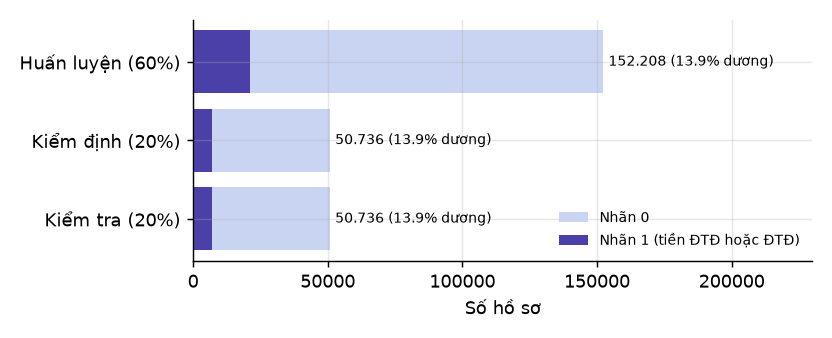
\includegraphics[width=0.78\textwidth]{images/fig_split.png}
\caption{Cách chia dữ liệu 60/20/20, phân tầng theo nhãn, \texttt{random\_state=42}}\label{fig:split}
\end{figure}
\nbcell{setup}{khởi tạo, nạp \texttt{metrics.json}, định dạng số kiểu Việt Nam}
\nbcell{split}{chia dữ liệu và vẽ Hình~\ref{fig:split}}


\subsection{Mô hình và huấn luyện}
Dữ liệu được chia thành tập huấn luyện (152.208), kiểm định (50.736) và kiểm tra (50.736) (Hình~\ref{fig:split}). Quy trình trong \code{models/training_pipeline.py}:
\begin{enumerate}[nosep]
\item Năm mô hình ứng viên: hồi quy logistic (đối chứng), rừng ngẫu nhiên, LightGBM, HistGradientBoosting và MLP PyTorch; tất cả dùng cân bằng lớp.
\item CV phân tầng 5 lần trên tập huấn luyện; hai mô hình có CV cao nhất được tuning bằng \code{RandomizedSearchCV} (12 vòng, \code{cv=3}).
\item MLP: các lớp ẩn $(64,32)$ với ReLU và Dropout $0{,}2$; hàm mất mát BCE có \code{pos_weight}; tối ưu AdamW \cite{adamw} ($\text{lr}=10^{-3}$, weight decay $10^{-5}$); dừng sớm theo mất mát kiểm định (patience 5). Đây là bộ tham số tốt nhất do tuning chọn.
\item Hiệu chuẩn xác suất bằng hồi quy đẳng điệu (\code{CalibratedClassifierCV}, \code{isotonic}, \code{cv=3}), vì cân bằng lớp làm lệch xác suất.
\item \textbf{Chọn mô hình và ngưỡng trên tập kiểm định}; tập kiểm tra chỉ dùng để đánh giá cuối.
\end{enumerate}

\begin{figure}[H]
\centering
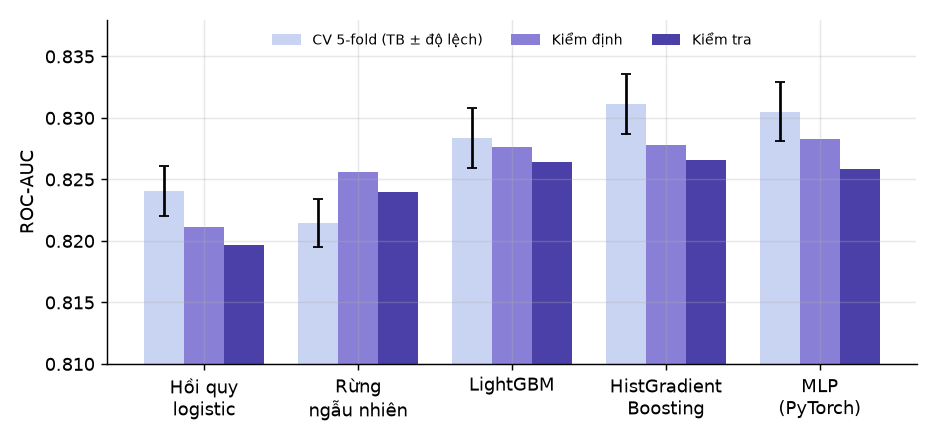
\includegraphics[width=0.92\textwidth]{images/fig_model_compare.png}
\caption{ROC-AUC của năm mô hình ứng viên (CV, kiểm định, kiểm tra), vẽ từ \texttt{metrics.json}}\label{fig:compare}
\end{figure}

\begin{table}[H]
\centering
\caption{Kết quả năm mô hình (ROC-AUC của CV là trung bình $\pm$ độ lệch chuẩn)}\label{tab:models}
\begin{tabular}{@{}lccccc@{}}
\toprule
\textbf{Mô hình} & \textbf{CV AUC} & \textbf{Kiểm định} & \textbf{Kiểm tra} & \textbf{AP (kiểm tra)} & \textbf{Brier}\\
\midrule
Hồi quy logistic & $0,8241\pm0,0020$ & 0,8211 & 0,8197 & 0,392 & 0,0993 \\
Rừng ngẫu nhiên & $0,8215\pm0,0020$ & 0,8256 & 0,8240 & 0,415 & 0,0980 \\
LightGBM & $0,8284\pm0,0024$ & 0,8276 & 0,8264 & 0,422 & 0,0975 \\
HistGradientBoosting & $0,8312\pm0,0024$ & 0,8278 & 0,8266 & 0,422 & 0,0974 \\
\textbf{MLP (được chọn)} & $0,8305\pm0,0024$ & 0,8283 & 0,8258 & 0,414 & 0,0978 \\
\bottomrule
\end{tabular}

\end{table}
\nbcell{compare}{vẽ Hình~\ref{fig:compare} và ghi Bảng~\ref{tab:models} ra \texttt{tables/tab\_models.tex}}


\textbf{Nhận xét thẳng thắn.} MLP được chọn vì có AUC kiểm định cao nhất (0,8283 so với 0,8278 của HistGradientBoosting), nhưng chênh lệch này nằm trong nhiễu; trên tập kiểm tra HistGradientBoosting thậm chí nhỉnh hơn (0,8266 so với 0,8258). Với 21 đặc trưng dạng bảng, các mô hình boosting và MLP tương đương, và hồi quy logistic chỉ kém khoảng 0,006 AUC. Dự án vẫn dùng MLP để đáp ứng khối ``Deep Learning'' của sơ đồ, chứ không phải vì học sâu vượt trội.

\begin{figure}[H]
\centering
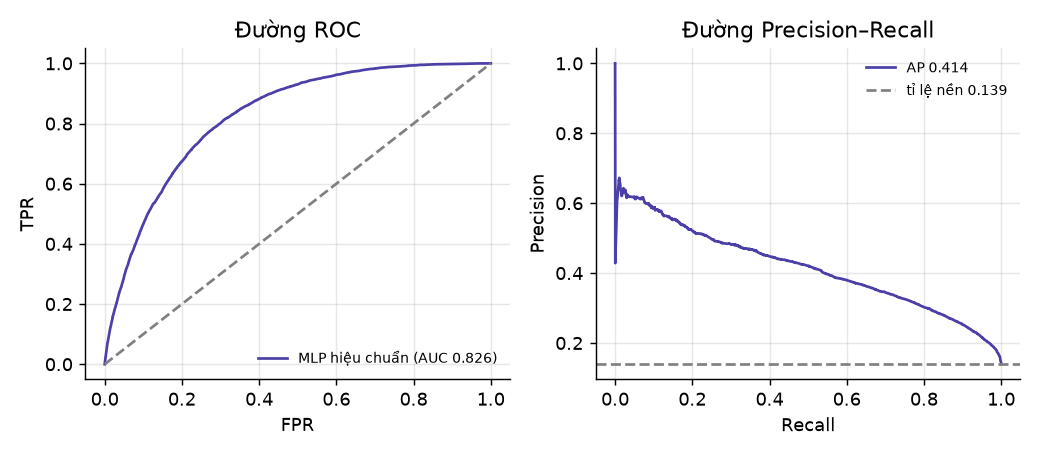
\includegraphics[width=\textwidth]{images/fig_roc_pr.png}
\caption{Đường ROC và Precision--Recall của MLP hiệu chuẩn trên tập kiểm tra}\label{fig:rocpr}
\end{figure}
\nbcell{rocpr}{vẽ Hình~\ref{fig:rocpr}}


\subsection{Hiệu chuẩn, ngưỡng và phân tầng nguy cơ}
Sau hiệu chuẩn, xác suất dự đoán khớp tỉ lệ dương thực tế (Hình~\ref{fig:calib}, Brier 0,0978). Hai khái niệm được tách riêng nhưng cùng chọn trên tập kiểm định:
\begin{itemize}[nosep]
\item \textbf{Ngưỡng nhị phân} $0{,}23906$: xác suất cho F1 cao nhất trên kiểm định; $\ge$ ngưỡng thì gắn cờ dương tính.
\item \textbf{Ba mức}: Thấp ($p<0{,}23906$), Trung bình ($0{,}23906\le p<0{,}40992$), Cao ($p\ge0{,}40992$), trong đó mốc Cao là xác suất thấp nhất trên kiểm định mà độ chính xác của các ca được gắn cờ đạt tối thiểu 0,5.
\end{itemize}
Nhờ vậy mọi ca dương tính đều từ mức Trung bình trở lên; trước đây mốc cố định 0,4/0,7 làm một ca xác suất 0,30 vừa dương tính vừa ``Thấp''. Trên tập kiểm tra, tỉ lệ nhãn 1 theo mức là 7,1\% (Thấp, 39.495 ca), 32,1\% (Trung bình, 7.371 ca) và 49,0\% (Cao, 3.870 ca), tức phân tầng có ý nghĩa. Tại ngưỡng 0,23906: độ chính xác 0,379, độ nhạy 0,603, F1 0,465 (Hình~\ref{fig:conf}).

\begin{figure}[H]
\centering
\begin{minipage}{0.47\textwidth}\centering
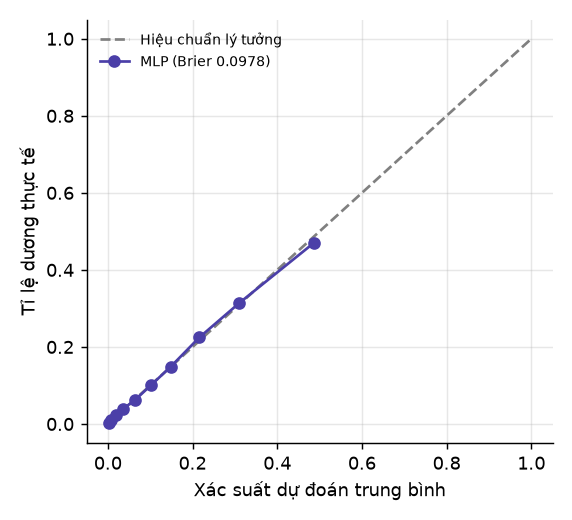
\includegraphics[width=\textwidth]{images/fig_calibration.png}
\caption{Đường hiệu chuẩn}\label{fig:calib}
\end{minipage}\hfill
\begin{minipage}{0.47\textwidth}\centering
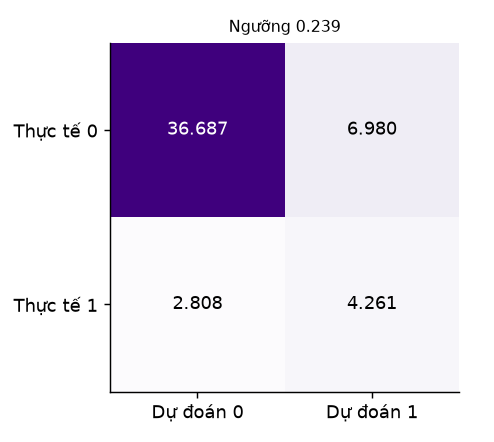
\includegraphics[width=0.9\textwidth]{images/fig_confusion.png}
\caption{Ma trận nhầm lẫn tại ngưỡng nhị phân}\label{fig:conf}
\end{minipage}
\end{figure}
\nbcell{calib}{vẽ Hình~\ref{fig:calib}}
\nbcell{confusion}{vẽ Hình~\ref{fig:conf}}


\begin{figure}[H]
\centering
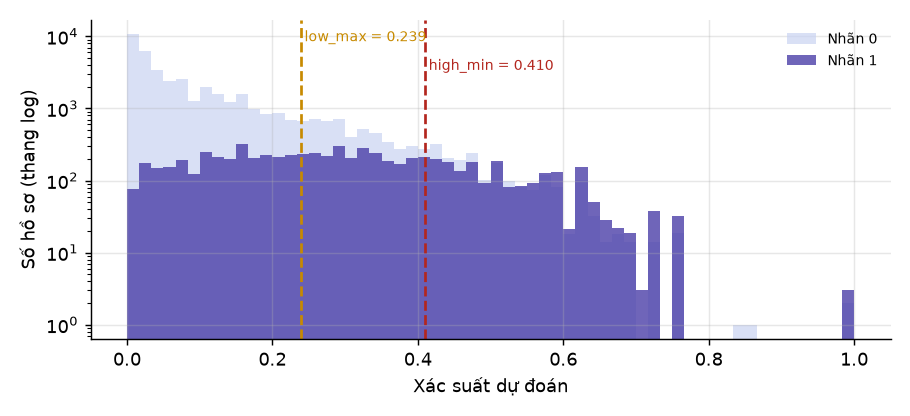
\includegraphics[width=0.9\textwidth]{images/fig_bands.png}
\caption{Phân bố xác suất theo nhãn và hai mốc phân tầng (thang log)}\label{fig:bands}
\end{figure}

\begin{table}[H]
\centering
\caption{Tỉ lệ nhãn 1 trên tập kiểm tra theo mức nguy cơ}\label{tab:bands}
\begin{tabular}{@{}lccc@{}}
\toprule
\textbf{Mức} & \textbf{Số ca} & \textbf{Nhãn 1} & \textbf{Tỉ lệ nhãn 1}\\
\midrule
Thấp & 39.495 & 2.808 & 7,1\% \\
Trung bình & 7.371 & 2.365 & 32,1\% \\
Cao & 3.870 & 1.896 & 49,0\% \\
\bottomrule
\end{tabular}

\end{table}
\nbcell{bands}{vẽ Hình~\ref{fig:bands} và ghi Bảng~\ref{tab:bands}}


\subsection{Từ mô hình thành thành phần của hệ thống}
Một con số xác suất chưa đủ để tư vấn. Quanh mô hình, \code{RiskModel} và \code{FeatureExplainer} bổ sung:
\begin{enumerate}[nosep]
\item \textbf{Chuẩn hóa đầu vào}: người dùng chỉ cần tuổi, huyết áp tâm thu và BMI (hoặc chiều cao, cân nặng); tuổi đổi thành nhóm BRFSS; \code{HighBP} suy ra từ huyết áp $\ge130$ mmHg nếu người dùng không khai (xấp xỉ, ghi rõ là hạn chế); các mục tùy chọn thiếu được điền giá trị mặc định và \textbf{được đánh dấu} (\code{defaulted_fields}).
\item \textbf{Giải thích}: phân tích độ nhạy, tức thay từng đặc trưng bằng giá trị mặc định (trung vị huấn luyện) rồi đo xác suất đổi bao nhiêu; trường tự điền bị đánh dấu để không giải thích như thể người dùng đã khai.
\item \textbf{Điểm chất lượng dữ liệu} (\code{confidence_score}): điểm quy ước trừ theo tỉ lệ mục tùy chọn bị tự điền (tối đa 0,2), huyết áp $\le70$ hoặc $\ge220$ mmHg ($-0{,}15$) và BMI $\le14$ hoặc $\ge50$ ($-0{,}1$). \emph{Đây không phải độ tin cậy thống kê}, và giao diện ghi rõ như vậy.
\item \textbf{Hồ sơ tương tự}: tìm theo khoảng cách số trên tuổi, BMI, huyết áp và glucose (khi cả hai đều đo); mỗi hồ sơ mang \code{outcome_confirmed = false}, tức là dự đoán cũ chứ không phải kết quả bệnh đã xác nhận.
\end{enumerate}

\section{Knowledge Base và RAG}
\subsection{Nguồn tri thức và đồ thị Neo4j}
Danh sách nguồn được cấu hình tại \code{data/corpus/sources.json}; các thực thể và quan hệ tuyển chọn nằm tại \code{data/corpus/graph.json}. Script \code{scripts/collect_corpus.py} thu thập web/PDF, chia đoạn bằng chứng, ghép đồ thị trong bộ nhớ, kiểm tra nhất quán rồi nạp trực tiếp vào Neo4j bằng \code{MERGE}. Nội dung y khoa \textbf{chưa được chuyên gia y khoa thẩm định}. Bản chụp cố định \code{tests/fixtures/diabetes_kb.json} phục vụ kiểm thử, đánh giá ngoại tuyến và báo cáo; \code{scripts/load_neo4j_kb.py} là công cụ khôi phục tùy chọn từ bản chụp này.

Lược đồ gồm bốn nhãn thực thể (\code{Condition}, \code{RiskFactor}, \code{Test}, \code{Intervention}), nút \code{Evidence} và \code{Source}, và năm loại quan hệ: \code{INCREASES_RISK_OF}, \code{DIAGNOSES}, \code{REDUCES_RISK_OF}, \code{ADDRESSES}, \code{SHOULD_TEST_WITH}. Mỗi quan hệ mang \code{evidence_ids}; mỗi \code{Evidence} nối tới \code{Source} qua \code{FROM}, nên mọi khẳng định truy vấn ra đều đi kèm trích dẫn. Kết quả: 20 thực thể, 35 quan hệ nghiệp vụ, 21 đoạn bằng chứng, 5 nguồn; sau khi nạp, Neo4j có 46 nút và 56 quan hệ (gồm 21 quan hệ bằng chứng $\rightarrow$ nguồn), được xác minh ngày 03/11/2026 trên Neo4j 2026.10.1 chạy trong Docker.

Hình~\ref{fig:kg} vẽ đồ thị tri thức từ bản chụp ngoại tuyến \code{tests/fixtures/diabetes_kb.json} bằng NetworkX; hình chỉ gồm 20 nút thực thể và 35 quan hệ, còn các nút \code{Evidence} và \code{Source} không được vẽ cho gọn. Bảng~\ref{tab:kb} thống kê số lượng, cùng cell sinh ra chúng.

\begin{figure}[H]
\centering
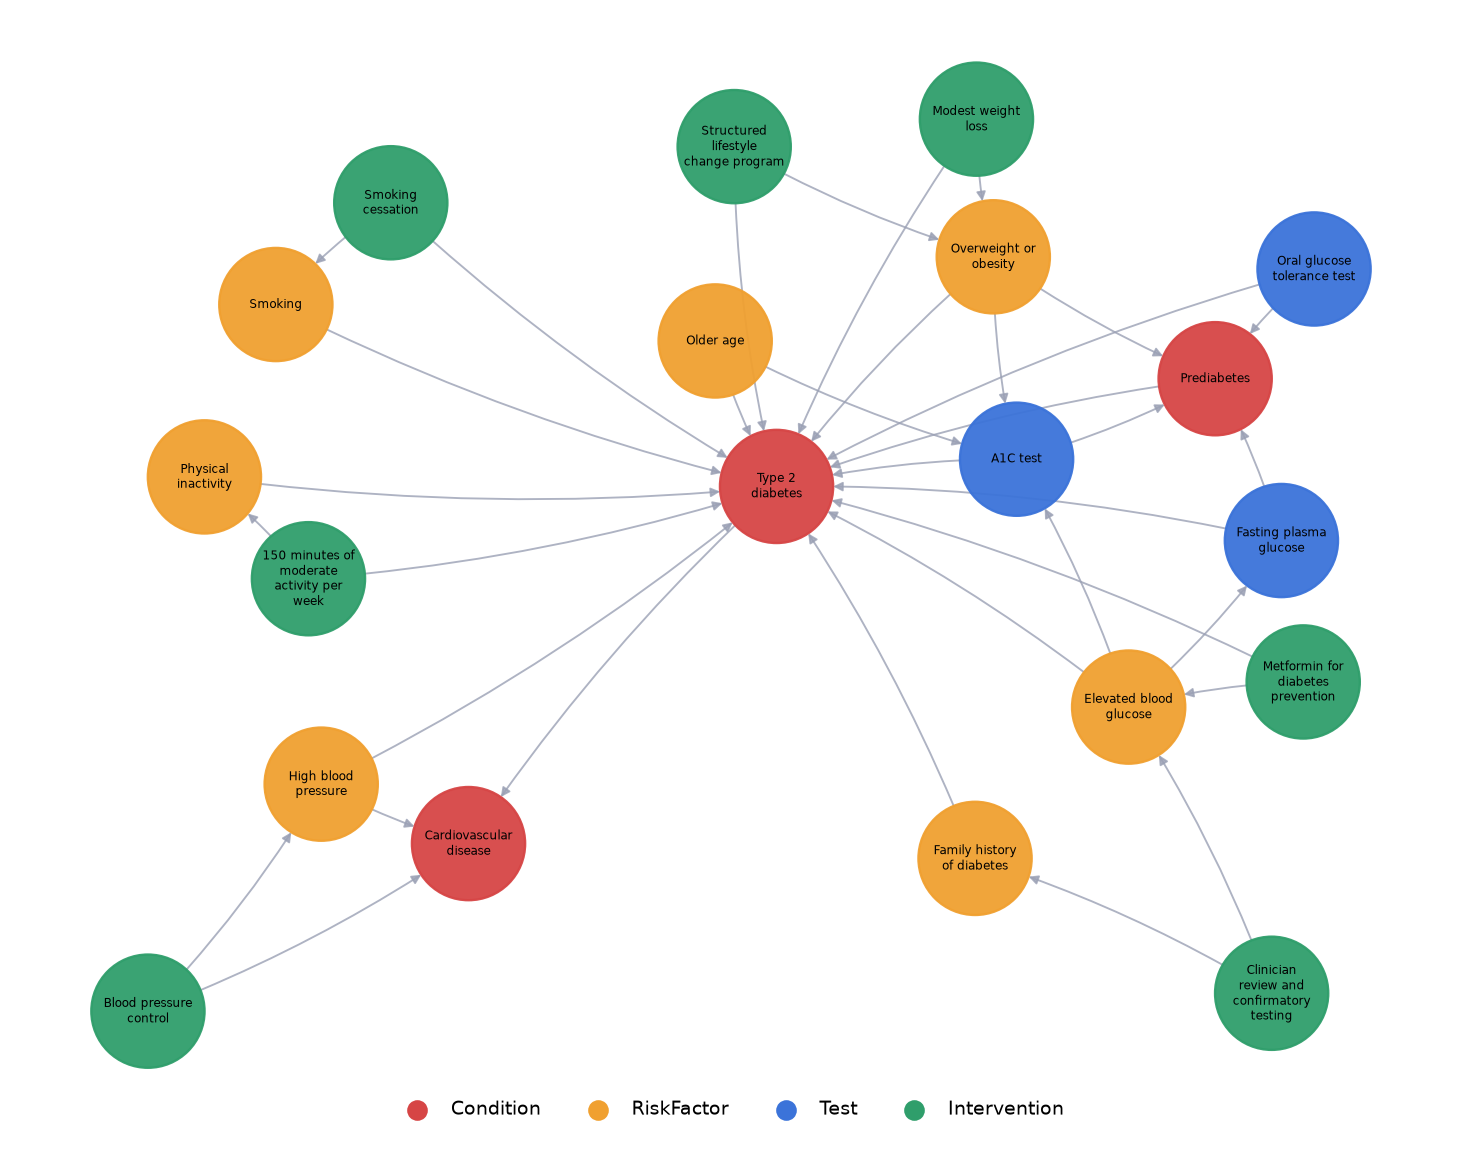
\includegraphics[width=0.95\textwidth]{images/fig_kg.png}
\caption{Đồ thị tri thức về ĐTĐ (nút tô màu theo nhãn: Condition, RiskFactor, Test, Intervention)}\label{fig:kg}
\end{figure}
\begin{table}[H]
\centering
\caption{Thống kê nút và quan hệ của KB}\label{tab:kb}
\begin{tabular}{@{}lr@{\hspace{2em}}lr@{}}
\toprule
\textbf{Nút / dữ liệu} & \textbf{SL} & \textbf{Loại quan hệ} & \textbf{SL}\\
\midrule
Condition & 3 & ADDRESSES & 8 \\
Intervention & 7 & DIAGNOSES & 6 \\
RiskFactor & 7 & INCREASES\_RISK\_OF & 11 \\
Test & 3 & REDUCES\_RISK\_OF & 6 \\
Đoạn bằng chứng & 21 & SHOULD\_TEST\_WITH & 4 \\
Nguồn & 5 & & \\
\bottomrule
\end{tabular}

\end{table}
\nbcell{kg}{vẽ Hình~\ref{fig:kg} và ghi Bảng~\ref{tab:kb}}

\subsection{Truy xuất: ngữ nghĩa kết hợp đồ thị}
\code{RetrievalAgent} thực hiện \cite{lewis2020}:
\begin{enumerate}[nosep]
\item Dựng câu truy vấn từ mức nguy cơ, các yếu tố nguy cơ có tác động dương trong giải thích, và việc glucose đã đo hay chưa.
\item Nhúng bằng \code{all-MiniLM-L6-v2} và tính độ tương đồng cosine với các đoạn bằng chứng trong ChromaDB (chỉ mục HNSW).
\item Loại đoạn có độ liên quan dưới \textbf{0,3}; đoạn mà đồ thị gắn với yếu tố nguy cơ của bệnh nhân được cộng \textbf{0,15} khi xếp hạng.
\item Gán \code{evidence_status}: \code{none} (không có đoạn nào), \code{limited} (dưới 2 đoạn hoặc đoạn tốt nhất dưới 0,45), \code{sufficient} (còn lại).
\end{enumerate}
Khi policy chọn ``tìm thêm bằng chứng'', agent chạy thêm một truy vấn hướng dẫn chung, giữ điểm tốt nhất của mỗi đoạn và trả tối đa 5 đoạn. Ứng dụng bắt buộc dùng Neo4j; nếu không kết nối được lúc khởi tạo hoặc chưa đặt \code{NEO4J_PASSWORD}, dịch vụ phân tích báo lỗi và không chuyển sang JSON. Tệp JSON vẫn là nguồn nạp/cập nhật đồ thị; \code{FileKnowledgeBase} chỉ được chọn tường minh cho kiểm thử và đánh giá ngoại tuyến.

\begin{lstlisting}[caption={Rút gọn RetrievalAgent.retrieve (agents/retriever.py)}]
factors = self._risk_factors(patient_data, feature_explanation)
queries = [self._query_text(patient_data, risk, factors)]
if broaden:                       # policy asked for more evidence
    queries.append(BROAD_QUERY)
    n_results = max(n_results, BROAD_N_RESULTS)
for query in queries:             # keep each passage's best cosine score
    res = self.collection.query(query_embeddings=[embed(query)], n_results=count)
    ...
linked = self._graph_links(factors)          # evidence_id -> graph rows (Neo4j)
for evidence_id, score in relevance.items():
    if score < self.min_relevance:           # 0.3
        continue
    ...  # "graph+semantic" if linked else "semantic"
contexts.sort(key=lambda c: c["relevance"] + (GRAPH_BOOST if c["supports"] else 0))
\end{lstlisting}

\textbf{Giới hạn đánh giá.} Dự án \textbf{chưa} có bộ câu hỏi đánh giá truy xuất có đáp án (không đo được hit@$k$ hay MRR). Các ngưỡng 0,3, 0,45 và 0,15 được đặt theo một số ca thử, chưa hiệu chỉnh trên tập đánh giá; kiểm thử hiện tại (\code{tests/test_retriever.py}) chỉ kiểm tra hành vi (không bằng chứng, bằng chứng hạn chế, thứ tự, dự phòng). Embedding MiniLM chủ yếu dành cho tiếng Anh, còn KB lưu bằng chứng tiếng Anh và có bản diễn đạt tiếng Việt để hiển thị.

\section{Bộ luật và Reinforcement Learning}
\subsection{Bộ luật an toàn và xử lý xung đột}
Bộ luật (\code{tools/rules.py}) chạy hai pha: luật \emph{cơ sở} xét số đo, dự đoán và chất lượng dữ liệu; luật \emph{xung đột} xét sự bất đồng giữa các kết quả đó và bằng chứng. Mỗi luật có mã, tên, nhóm, mức ưu tiên (số lớn hơn quan trọng hơn), điều kiện, thông điệp, mức chuyển tuyến và căn cứ. Các ngưỡng là \emph{ngưỡng của dự án}, có đối chiếu với ADA và khuyến cáo ACC/AHA \cite{whelton2018}, \textbf{chưa được bác sĩ thẩm định}.

\begin{table}[H]
\centering
\caption{Các luật hiện có trong \texttt{tools/rules.py}}\label{tab:rules}
\begin{tabularx}{\textwidth}{@{}L{3.6cm}c L{4.6cm}X@{}}
\toprule
\textbf{Mã luật} & \textbf{Ưu tiên} & \textbf{Điều kiện} & \textbf{Hướng xử trí}\\
\midrule
\code{GLU-300} & 100 & Glucose đo được $\ge300$ mg/dL & Khám khẩn cấp\\
\code{BP-180} & 95 & Huyết áp tâm thu $\ge180$ mmHg & Khám khẩn cấp\\
\code{GLU-200} & 80 & Glucose đo được 200--299 & Sớm khám bác sĩ\\
\code{BP-160} & 75 & Huyết áp tâm thu 160--179 & Sớm khám bác sĩ\\
\code{PRED-VERYHIGH} & 60 & Mức Cao và $p\ge0{,}85$ & Sớm khám bác sĩ\\
\midrule
\code{CF-PRED-LOW-MEASURED-HIGH} & 85 & Mô hình Thấp nhưng có số đo nguy hiểm & Số đo thắng; \code{effective_risk}=Cao\\
\code{CF-PRED-HIGH-GLUCOSE-NORMAL} & 55 & Mô hình Cao nhưng glucose đo $<100$ & Giữ mức Cao, đề nghị A1C\\
\code{CF-PRED-HIGH-LOW-QUALITY} & 40 & Mô hình Cao trên dữ liệu chất lượng thấp & Đánh dấu tạm thời\\
\code{CF-ESCALATION-NO-EVIDENCE} & 30 & Có chuyển tuyến nhưng bằng chứng \code{none}/\code{limited} & Không hạ mức chuyển tuyến\\
\bottomrule
\end{tabularx}
\end{table}

Chính sách giải quyết: (1) số đo lâm sàng thắng dự đoán thống kê, khuyến nghị viết theo \code{effective_risk}; (2) mức chuyển tuyến là mức nặng nhất trong các luật đã kích hoạt, không gì hạ được, kể cả dự đoán thấp hay thiếu bằng chứng; (3) mọi xung đột đều được báo cáo kèm cách giải quyết, không bị ẩn. Luật glucose chỉ áp dụng cho giá trị \emph{đo thật}, không dùng giá trị điền thay thế. Việc chưa đo glucose \textbf{không} còn là luật cảnh báo riêng: thay vào đó giao diện hỏi bổ sung (Mục~4.4).

\subsection{Agent chọn bước hỗ trợ bằng Q-learning}
Policy (\code{rl/}) mô hình hóa việc chọn bước tiếp theo như một MDP; Q-learning \cite{watkins1992,sutton2018} cập nhật $Q(s,a)\leftarrow Q(s,a)+\alpha\,[\,r+\gamma\max_{a'}Q(s',a')-Q(s,a)\,]$ với $\alpha=0{,}1$ và $\gamma=1$ (bài toán có kết thúc hữu hạn).
\begin{itemize}[nosep]
\item \textbf{Trạng thái} (108 = $3\times3\times3\times2\times2$): mức nguy cơ (Thấp/Trung bình/Cao); glucose (chưa đo/bình thường/$\ge200$); \code{evidence_status}; đã hỏi glucose chưa; đã tìm mở rộng chưa.
\item \textbf{Hành động} (5): \code{request_glucose}, \code{retrieve_more_evidence} (mỗi bước tối đa một lần), và ba bước kết thúc \code{recommend_routine}, \code{recommend_followup}, \code{escalate_to_clinician}.
\item \textbf{Phần thưởng}: mỗi bước thu thập $-0{,}05$; bước kết thúc $+1$ nếu đúng mức cần, phạt khi sai, nặng nhất khi bỏ sót ca cần chuyển tuyến ($-2$), nhẹ khi chuyển tuyến thừa ($-0{,}4$ đến $-0{,}8$); lời khuyên không chuyển tuyến cộng $+0{,}2$ nếu bằng chứng đủ, trừ $0{,}2$ nếu không có.
\item \textbf{Huấn luyện}: 60.000 tập, $\epsilon$ giảm tuyến tính từ 1 xuống 0,05 trong 80\% số tập đầu.
\end{itemize}
\textbf{Hạn chế cần nói rõ.} Môi trường, xác suất bệnh nhân cung cấp glucose, khả năng tìm mở rộng cải thiện bằng chứng (giả định 60\%) và mọi giá trị phần thưởng đều do nhóm đặt, ghi trong \code{rl/environment.py}; \textbf{không có phản hồi thật} từ bệnh nhân hay bác sĩ. Kết quả chỉ cho biết các chiến lược khác nhau ra sao \emph{dưới các giả định đó}.

\begin{table}[H]
\centering
\caption{So sánh chiến lược trên 20.000 tập mô phỏng}\label{tab:rl}
\begin{tabular}{@{}lcccc@{}}
\toprule
\textbf{Chiến lược} & \textbf{Reward TB $\pm$ 95\% CI} & \textbf{Số bước} & \textbf{Bỏ sót} & \textbf{Chuyển thừa}\\
\midrule
Q-learning & $0,956\pm0,005$ & 1,78 & 0,65\% & 3,55\% \\
Bảng kiểm cố định & $0,946\pm0,006$ & 2,10 & 2,34\% & 0,00\% \\
Chỉ theo mức rủi ro & $0,803\pm0,011$ & 1,00 & 7,42\% & 0,00\% \\
Ngẫu nhiên & $-0,367\pm0,016$ & 1,28 & 26,47\% & 20,09\% \\
\bottomrule
\end{tabular}

\end{table}
\begin{figure}[H]
\centering
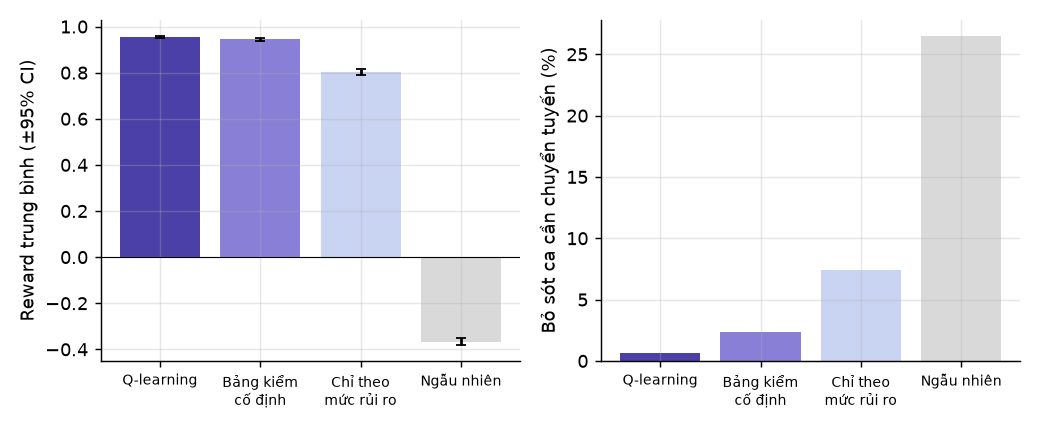
\includegraphics[width=0.9\textwidth]{images/fig_rl_compare.png}
\caption{Reward trung bình và tỉ lệ bỏ sót ca cần chuyển tuyến của bốn chiến lược (mô phỏng)}\label{fig:rl}
\end{figure}
\nbcell{rl}{vẽ Hình~\ref{fig:rl} và ghi Bảng~\ref{tab:rl}}

Q-learning và bảng kiểm cố định chênh nhau trong khoảng sai số, nên \textbf{không thể nói RL tốt hơn bảng kiểm}; cả hai vượt rõ quy trình chỉ theo mức rủi ro. Policy học được dùng ít bước hơn và bỏ sót ít hơn, đổi lại chuyển tuyến thừa nhiều hơn, và kết quả phụ thuộc vào ma trận phần thưởng.

\subsection{Luật ràng buộc chính sách học được}
Orchestrator dựng trạng thái sau lượt xử lý đầu và hỏi policy tối đa 3 bước. Chỉ ``tìm thêm bằng chứng'' được thực thi thật (chạy lại truy xuất mở rộng, luật và khuyến nghị); ``hỏi glucose'' không thực hiện được trong một lời gọi API nên chỉ trả về làm \code{policy.next_step}. \textbf{Luật luôn thắng}: nếu policy chọn bước thấp hơn mức luật đã yêu cầu, \code{next_step} bị thay bằng \code{escalate_to_clinician} và \code{overridden_by_rules = true}; policy không bao giờ thay đổi kết quả \code{safety}.

\section{Tư vấn, trợ giúp và cô lập lỗi}
\textbf{Khuyến nghị có nguồn.} \code{RecommendationAgent} chỉ dùng các đoạn bằng chứng đã đánh số, trích dẫn \code{[n]} kèm danh sách nguồn, và nói rõ khi thiếu bằng chứng thay vì bịa nguồn. Với \code{effective_risk} nâng lên do số đo, khuyến nghị viết theo mức đã nâng.

\textbf{Thang chỉ số và câu hỏi bổ sung.} API trả \code{measurement_scales} (BMI, huyết áp tâm thu, glucose) cùng vùng tham khảo có nguồn (CDC, AHA, NIDDK). Thang glucose chỉ có vùng tham khảo khi người dùng xác nhận đo lúc đói; huyết áp chỉ có số tâm thu nên không kết luận ``bình thường''; BMI chỉ phân vùng người lớn từ 20 tuổi. Hệ thống trả tối đa một \code{followup}: trước hết là glucose còn thiếu, sau đó là mục chưa khai mà câu trả lời làm xác suất MLP đổi nhiều nhất (chênh tối thiểu 2 điểm phần trăm). Mục đã trả lời hoặc đã bấm ``Bỏ qua'' không bị hỏi lại, và khi luật yêu cầu bác sĩ thì không đưa nhiệm vụ nhập liệu lên trước.

\textbf{Mô phỏng ``nếu thay đổi''} (\code{WhatIfSimulator}) tính lại xác suất khi giảm 5\% cân nặng (nếu BMI $\ge25$), vận động đều, bỏ thuốc lá, hoặc đưa huyết áp tâm thu xuống dưới 130 mmHg, chỉ với yếu tố mà người dùng \emph{thực sự khai} và có thể thay đổi, và gắn bằng chứng cho từng kịch bản. Chỉ chạy khi mức chuyển tuyến là theo dõi định kỳ.

\textbf{Trao đổi giữa các thành phần.} Khi các kết luận bất đồng, hệ thống ghi lại một đoạn hội thoại có kiểu (\code{agents/dialogue.py}, trường \code{trace.dialogue}). Mỗi thông điệp có người gửi, người nhận, performative, nội dung và vị trí trong luồng (\code{after_step}: số bước đã chạy khi thông điệp được gửi), nên giao diện xen hội thoại đúng chỗ trong dòng thời gian các bước thay vì tách thành một khối riêng; \code{SafetyGuard} gửi \code{challenge} tới thành phần mà một luật xung đột (hoặc việc ghi đè policy) làm mất hiệu lực, và người nhận trả lời bằng hàm phản hồi của chính nó (Bảng~\ref{tab:dialogue}). Mô hình \emph{chấp nhận} khi số đo thực tế thắng, nhưng \emph{giữ nguyên và đề xuất} xét nghiệm A1C khi glucose bình thường mà dự đoán vẫn cao, vì glucose không phải đặc trưng của mô hình. \code{RetrievalAgent} \emph{đề xuất} tìm mở rộng bằng chứng; đây là đề xuất duy nhất mà Orchestrator \textbf{thực hiện thật}: nó chạy lại truy xuất mở rộng, bộ luật và khuyến nghị (tối đa một lần, trước khi policy chạy), rồi \code{RetrievalAgent} báo kết quả bằng \code{inform} (số đoạn bằng chứng, trạng thái bằng chứng, hoặc lỗi nếu tìm thất bại và giữ nguyên các đoạn cũ).

\begin{table}[H]
\centering
\caption{Các cuộc trao đổi giữa thành phần (\texttt{agents/dialogue.py})}\label{tab:dialogue}
\begin{tabularx}{\textwidth}{@{}L{4.2cm}L{3.3cm}X@{}}
\toprule
\textbf{Nguyên nhân} & \textbf{Người bị thách thức} & \textbf{Phản hồi}\\
\midrule
\code{CF-PRED-LOW-MEASURED-HIGH} & \code{RiskModel} & \code{accept}: nâng nguy cơ hiệu lực lên Cao theo số đo\\
\code{CF-PRED-HIGH-GLUCOSE-NORMAL} & \code{RiskModel} & \code{propose}: giữ mức Cao, đề nghị xét nghiệm A1C\\
\code{CF-PRED-HIGH-LOW-QUALITY} & \code{RiskModel} & \code{accept}: đánh dấu dự đoán là tạm thời\\
\code{CF-ESCALATION-NO-EVIDENCE} & \code{RetrievalAgent} & \code{propose} tìm mở rộng (\textbf{được thực hiện}); sau đó \code{inform} kết quả\\
Luật ghi đè bước của policy & \code{QPolicy} & \code{accept}: chấp nhận bị ghi đè, chuyển bác sĩ\\
\bottomrule
\end{tabularx}
\end{table}

Cần nói thẳng về phạm vi của cơ chế này:
\begin{itemize}[nosep]
\item Các hàm phản hồi là \emph{tất định} và được viết sẵn, không có LLM và không có nhiều vòng thương lượng.
\item Chỉ một loại thông điệp \textbf{có tác động}: đề xuất tìm mở rộng. Nó đổi tập bằng chứng, trạng thái bằng chứng, khuyến nghị và trích dẫn, và có thể làm luật \code{CF-ESCALATION-NO-EVIDENCE} hết kích hoạt. Nó \emph{không} thể hạ mức chuyển tuyến, vì mức này do các luật cơ sở quyết định và các luật cơ sở không đọc bằng chứng.
\item Các thông điệp còn lại (phản hồi của \code{RiskModel} và \code{QPolicy}) chỉ \textbf{ghi lại lý do luật thắng}: mức nguy cơ hiệu lực và việc ghi đè policy do bộ luật quyết định, không phải do cuộc trao đổi.
\item Với KB hiện tại (21 đoạn bằng chứng), các hồ sơ thử đều có bằng chứng đủ, nên đề xuất tìm mở rộng \textbf{chưa kích hoạt trên dữ liệu thật}; hành vi này mới được kiểm chứng bằng kiểm thử với retriever giả cho kết quả yếu ở lần tìm đầu (\code{tests/test_dialogue.py}).
\end{itemize}
Đây là bản tối thiểu của giao tiếp agent--agent, đủ để truy vết ``ai phản biện ai, vì sao, và việc gì đã được làm theo'', chưa phải một giao thức thương lượng đầy đủ.

\textbf{Cô lập lỗi.} Mỗi bước tùy chọn chạy trong \code{RunLog.guard}; lỗi được ghi vào \code{degraded}, bước đó dùng nội dung dự phòng, và lời cảnh báo ``kết quả chưa đầy đủ'' được thêm vào \code{disclaimers}. Riêng bộ luật: nếu lỗi, kết quả nghiêng về \code{prompt_clinician_followup} với độ tin cậy Thấp, \emph{không} coi là an toàn. Lỗi mô hình trả HTTP 500, không tạo xác suất giả.

% ================= CHƯƠNG 5 =================
\chapter{CODE VÀ DEMO}

\section{Cấu trúc mã nguồn}
\begin{lstlisting}[caption={Cấu trúc thư mục chính của dự án}]
healthcare-agent-system/
|-- main.py              build_agent(): nap model, KB, memory, policy
|-- api/app.py           FastAPI: /v1/predict, /history, /health, xac thuc Bearer
|-- agents/              orchestrator, dialogue, retriever, explainer, recommender
|-- models/              risk_model.py, mlp.py (PyTorch->NumPy), training_pipeline.py
|-- rl/                  environment.py (mo phong), policy.py (Q-learning)
|-- tools/               rules.py, safety.py, neo4j_kb.py, explainability.py,
|                        what_if.py, patient_guidance.py, audit_logger.py
|-- memory/store.py      MemoryAgent (ChromaDB)
|-- data/                corpus/, training/ (BRFSS 2015 CSV), chroma/
|-- evaluation/          retrieval_questions.json
|-- artifacts/           risk_model.joblib, metrics.json, support_policy.json
|-- scripts/             download_training_data, train_diabetes_model,
|                        train_support_policy, load_neo4j_kb, demo_step12
|-- web/                 Next.js: app/, components/risk-console/, lib/
|-- ui/app.py            ban Streamlit
|-- tests/               154 kiem thu tu dong
|-- docs/, infra/aws/    tai lieu, Terraform App Runner
\end{lstlisting}

\section{Các hàm chính}
\begin{table}[H]
\centering
\caption{Các hàm và lớp chính}\label{tab:funcs}
\begin{tabularx}{\textwidth}{@{}L{5.4cm}X@{}}
\toprule
\textbf{Hàm / lớp} & \textbf{Vai trò}\\
\midrule
\code{Orchestrator.run} & Điều phối một lượt đánh giá, ghi \code{trace}, trả kết quả có cấu trúc\\
\code{Orchestrator._choose_next_step} & Vòng policy tối đa 3 bước; áp quyền ưu tiên của luật\\
\code{Orchestrator._negotiate} & Gửi \code{challenge} theo luật xung đột, thực hiện đề xuất tìm mở rộng của retriever (một lần), ghi kết quả bằng \code{inform}\\
\code{conflict_exchanges}, \code{override_exchange} & Dựng các thông điệp \code{challenge}/\code{accept}/\code{propose}/\code{inform} giữa các thành phần bất đồng\\
\code{RunLog.guard} & Bọc một bước tùy chọn: lỗi thành \code{degraded} và nội dung dự phòng\\
\code{RiskModel.assess} & Chuẩn hóa hồ sơ, ghi trường tự điền, trả xác suất đã hiệu chuẩn\\
\code{train_production_model} & CV, tuning, hiệu chuẩn, chọn mô hình và ngưỡng trên kiểm định\\
\code{TorchMLPClassifier} & MLP huấn luyện bằng PyTorch, suy luận bằng NumPy\\
\code{FeatureExplainer.explain} & Phân tích độ nhạy theo từng đặc trưng\\
\code{RetrievalAgent.retrieve} & Truy xuất ngữ nghĩa + liên kết đồ thị, tính \code{relevance}\\
\code{KnowledgeGraph} & Truy vấn Neo4j: \code{support_for_risk_factors}, \code{all_evidence}\\
\code{RuleEngine.evaluate} & Luật cơ sở rồi luật xung đột; trả \code{escalation}, \code{effective_risk}\\
\code{SafetyGuard.assess} & Chạy bộ luật và tính điểm chất lượng dữ liệu\\
\code{QPolicy.decide} & Chọn hành động theo bảng Q cho trạng thái hợp lệ\\
\code{WhatIfSimulator.scenarios} & Tính lại xác suất cho các kịch bản thay đổi\\
\code{build_followup} & Chọn một câu hỏi bổ sung theo thứ tự ưu tiên\\
\bottomrule
\end{tabularx}
\end{table}

\begin{lstlisting}[caption={Orchestrator: bước tùy chọn không làm hỏng cả yêu cầu (rút gọn)}]
retrieved = log.guard("retriever",
    lambda: self.retriever.retrieve(patient, risk, feature_explanation, broaden=broaden),
    list(previous),                       # fallback: keep earlier passages
    detail=lambda v: f"{len(v)} evidence passages",
    on_failure="keep previous passages")
# a failed rule check must not read as "all clear": fail toward clinician review
safety = log.guard("safety_guard",
    lambda: self.safety_guard.assess(patient, prob, risk, evidence_status=status),
    {"escalation": "prompt_clinician_followup", "confidence_label": "Low", ...})
\end{lstlisting}

\section{Cách chạy}
\begin{lstlisting}[caption={Cài đặt và chạy hệ thống (PowerShell)}]
.\.venv\Scripts\python.exe -m pip install -r requirements.txt
.\.venv\Scripts\python.exe scripts/download_training_data.py   # BRFSS 2015
.\.venv\Scripts\python.exe scripts/train_diabetes_model.py      # artifacts/
.\.venv\Scripts\python.exe scripts/train_support_policy.py      # policy Q-learning
docker compose up -d neo4j                                       # tuy chon
.\.venv\Scripts\python.exe scripts/load_neo4j_kb.py              # nap KB vao Neo4j
.\.venv\Scripts\python.exe -m uvicorn api.app:app --reload --env-file .env
cd web; npm ci; npm run dev                                      # http://localhost:3000
.\.venv\Scripts\python.exe -m pytest -q                          # kiem thu
\end{lstlisting}
Biến môi trường chính: \code{NEO4J_PASSWORD} (đặt thì dùng Neo4j, không thì đọc KB từ tệp), \code{OPENAI_API_KEY} (tùy chọn), \code{REQUIRE_API_TOKEN} và \code{API_TOKEN} (xác thực Bearer).

\section{Demo: giao diện web}
Giao diện web (Next.js) dẫn người dùng qua các câu hỏi ngắn rồi trình bày kết quả. Mỗi nhóm thành phần phía API được thể hiện bằng một ``nhân vật'' để người xem biết \emph{ai làm gì}: \textbf{Bé Tiếp} (tiếp đón, hỏi hồ sơ), \textbf{Ông Mô} (mô hình dự đoán, giải thích), \textbf{Bà Nhớ} (bộ nhớ hồ sơ tương tự), \textbf{Cô Chứng} (truy xuất bằng chứng), \textbf{Chú Luật} (luật an toàn) và \textbf{Bạn Gợi} (khuyến nghị, \emph{what-if}, policy). Phần cuối trang hiển thị \code{trace} của lượt xử lý dưới dạng dòng thời gian các bước; khi các thành phần bất đồng, cuộc trao đổi giữa các nhân vật xen vào ngay sau bước sinh ra nó (ảnh chụp dưới đây là bản giao diện trước khi thêm phần hội thoại). Hình~\ref{fig:ui1} là màn nhập hồ sơ, Hình~\ref{fig:ui2a}--\ref{fig:ui2d} là trang kết quả của hồ sơ mẫu (nữ 45 tuổi, 170 cm, 82,4 kg, huyết áp tâm thu 130 mmHg).

\begin{figure}[H]
\centering
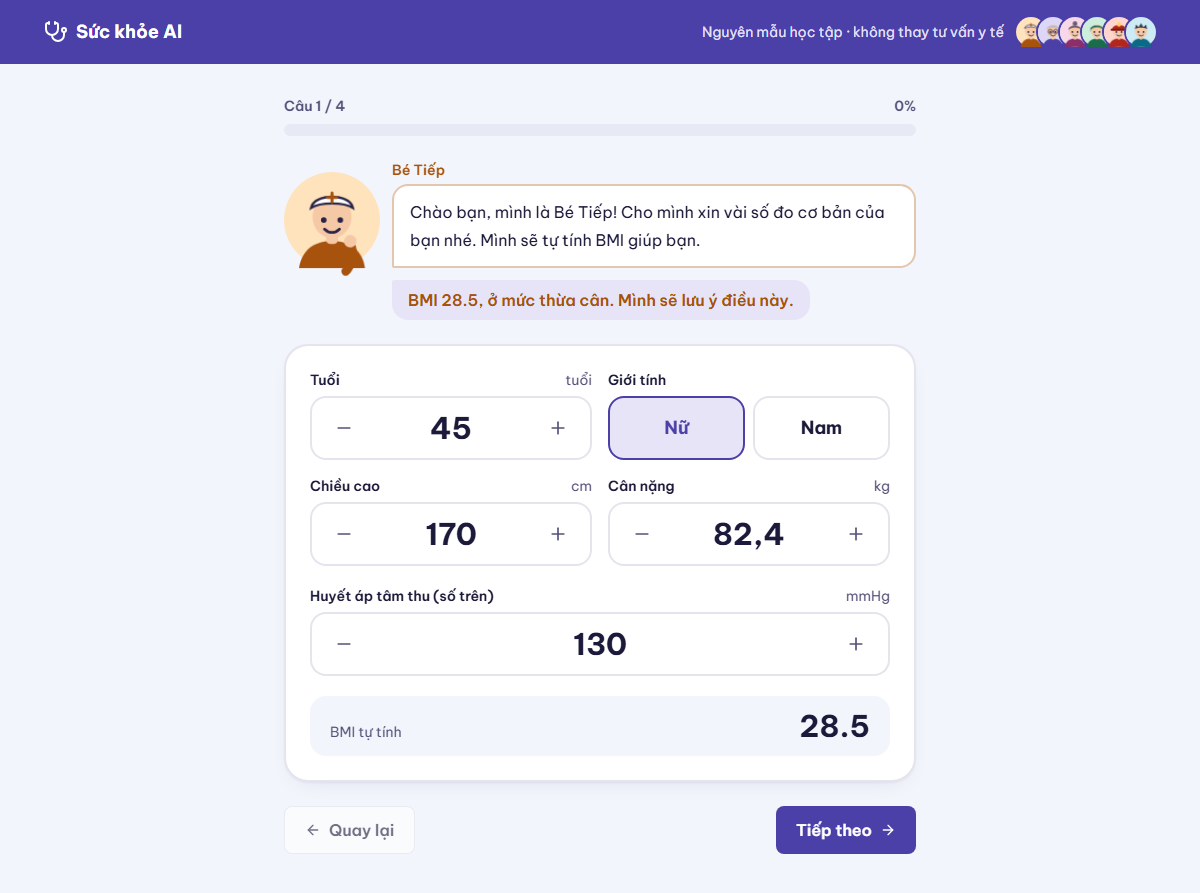
\includegraphics[width=0.62\textwidth]{images/ui_1.png}
\caption{Màn nhập hồ sơ: Bé Tiếp hỏi số đo cơ bản và tự tính BMI}\label{fig:ui1}
\end{figure}
\begin{figure}[H]
\centering
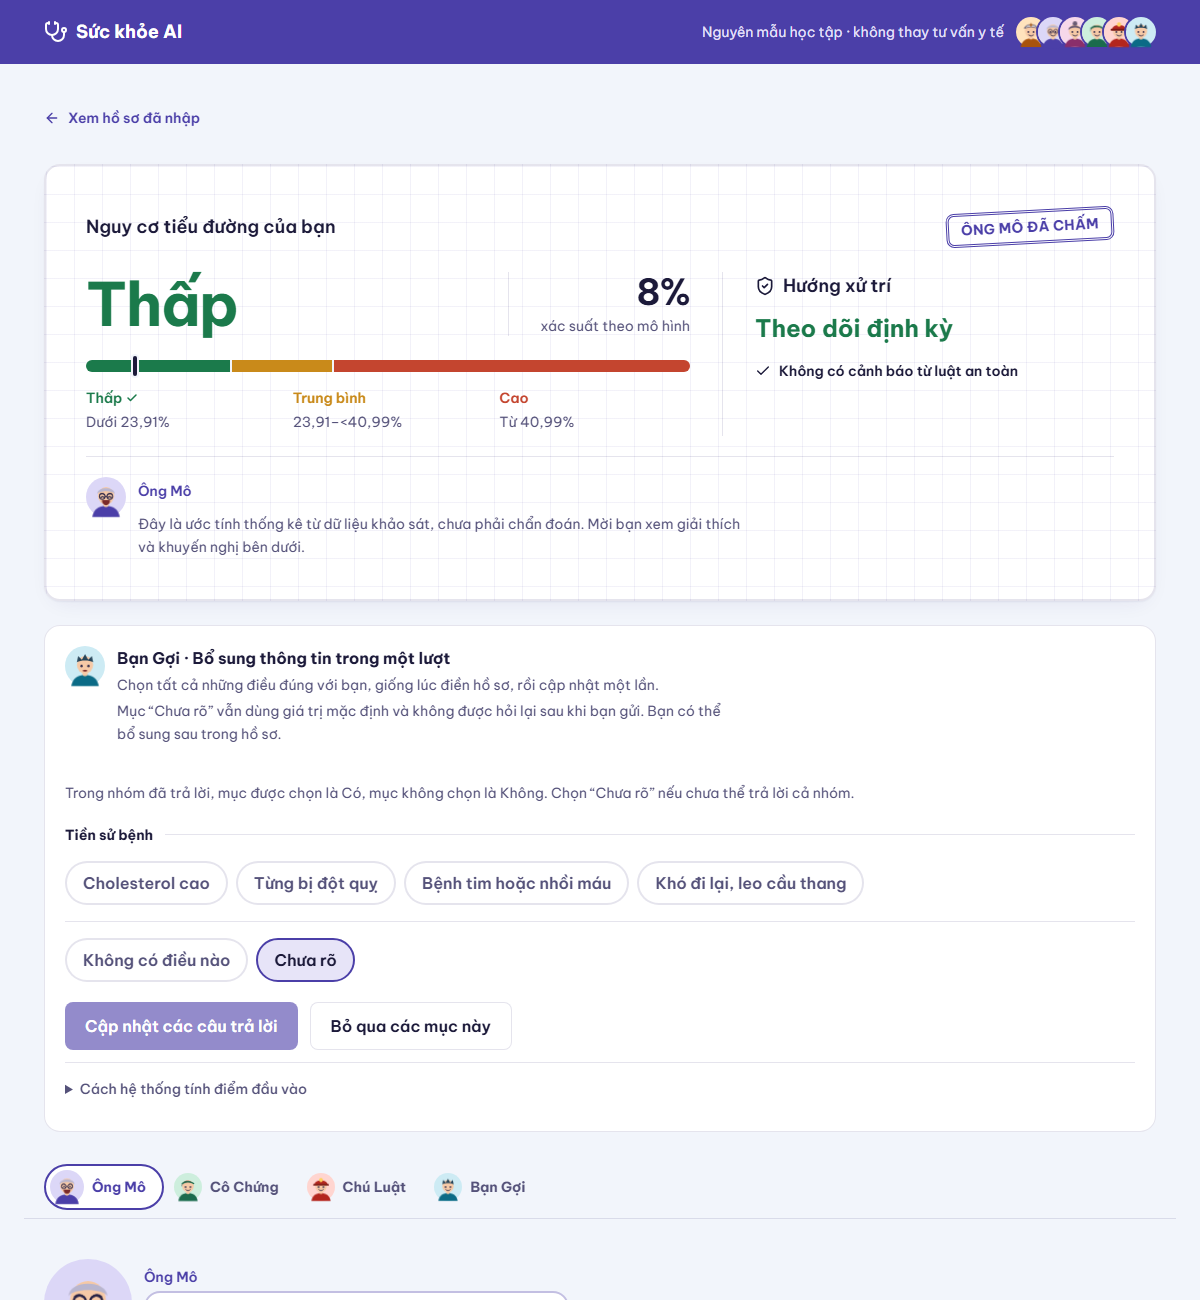
\includegraphics[width=\textwidth]{images/ui_2a.png}
\caption{Kết quả: mức nguy cơ, hướng xử trí và câu hỏi bổ sung theo nhóm}\label{fig:ui2a}
\end{figure}
\begin{figure}[H]
\centering
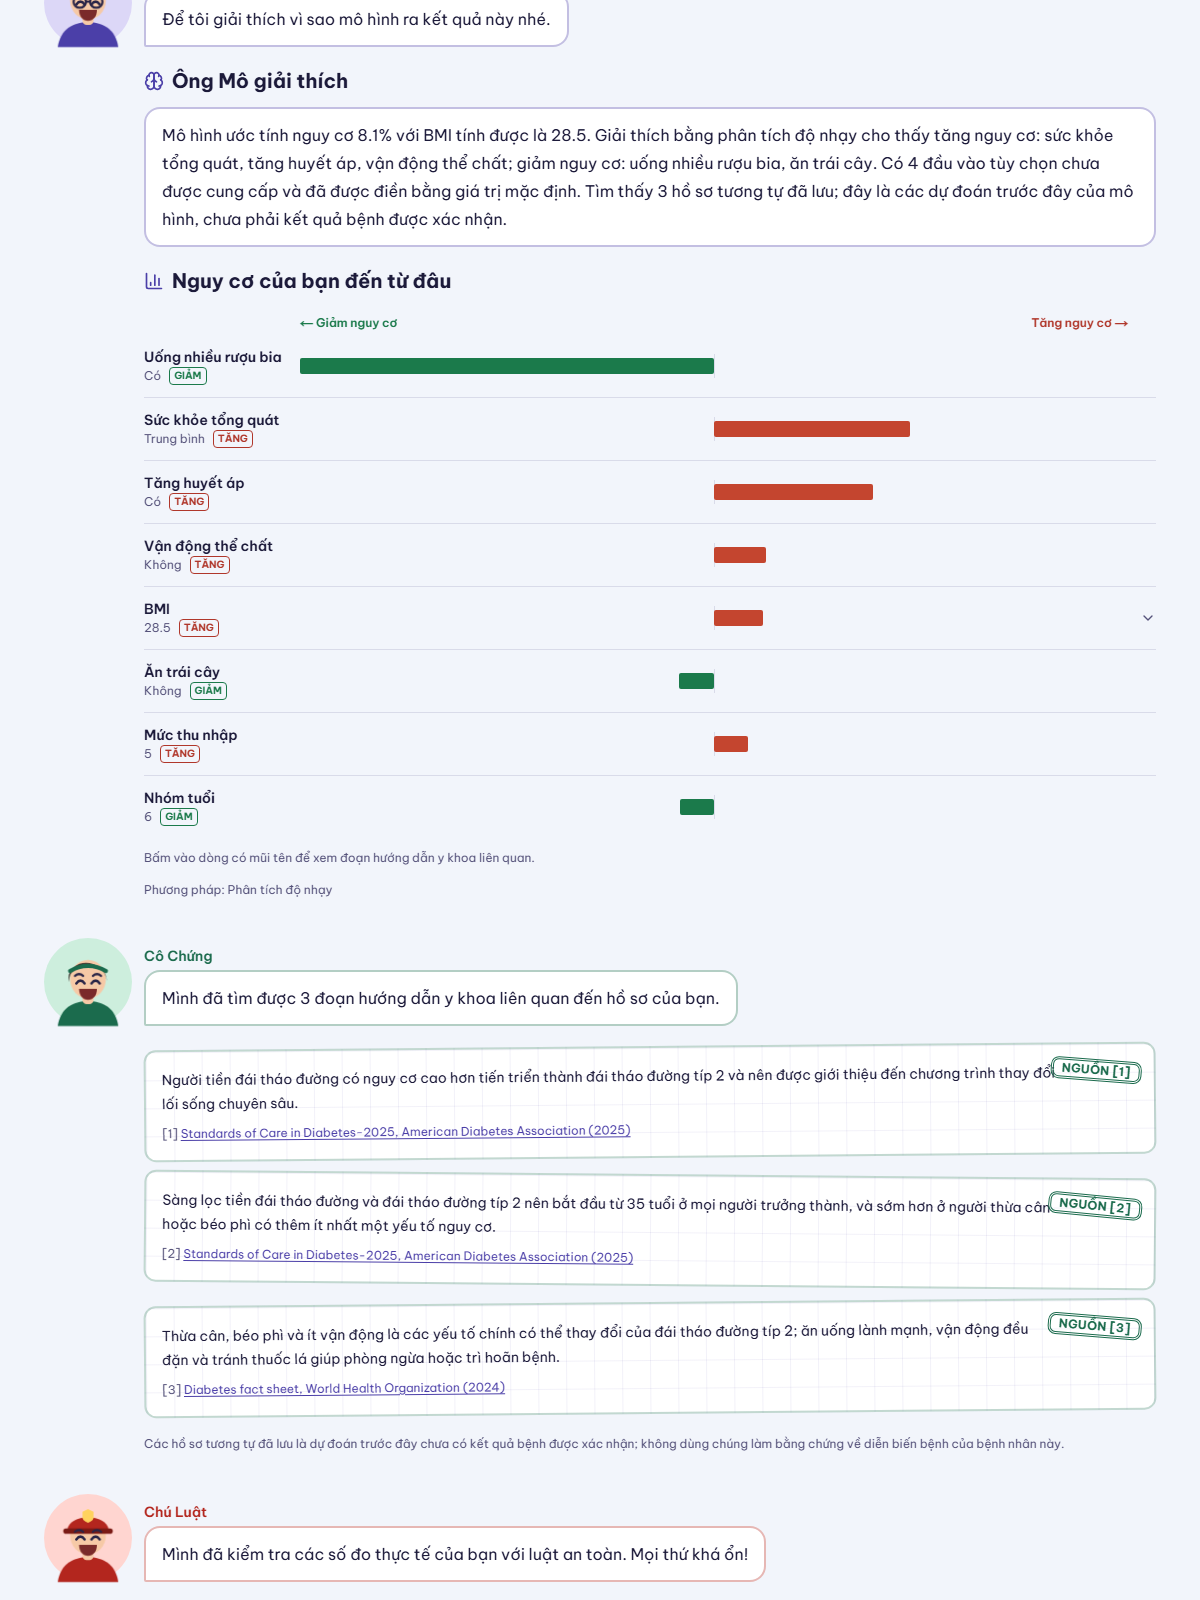
\includegraphics[width=0.92\textwidth]{images/ui_2b.png}
\caption{Ông Mô giải thích kết quả và biểu đồ tác động của đặc trưng}\label{fig:ui2b}
\end{figure}
\begin{figure}[H]
\centering
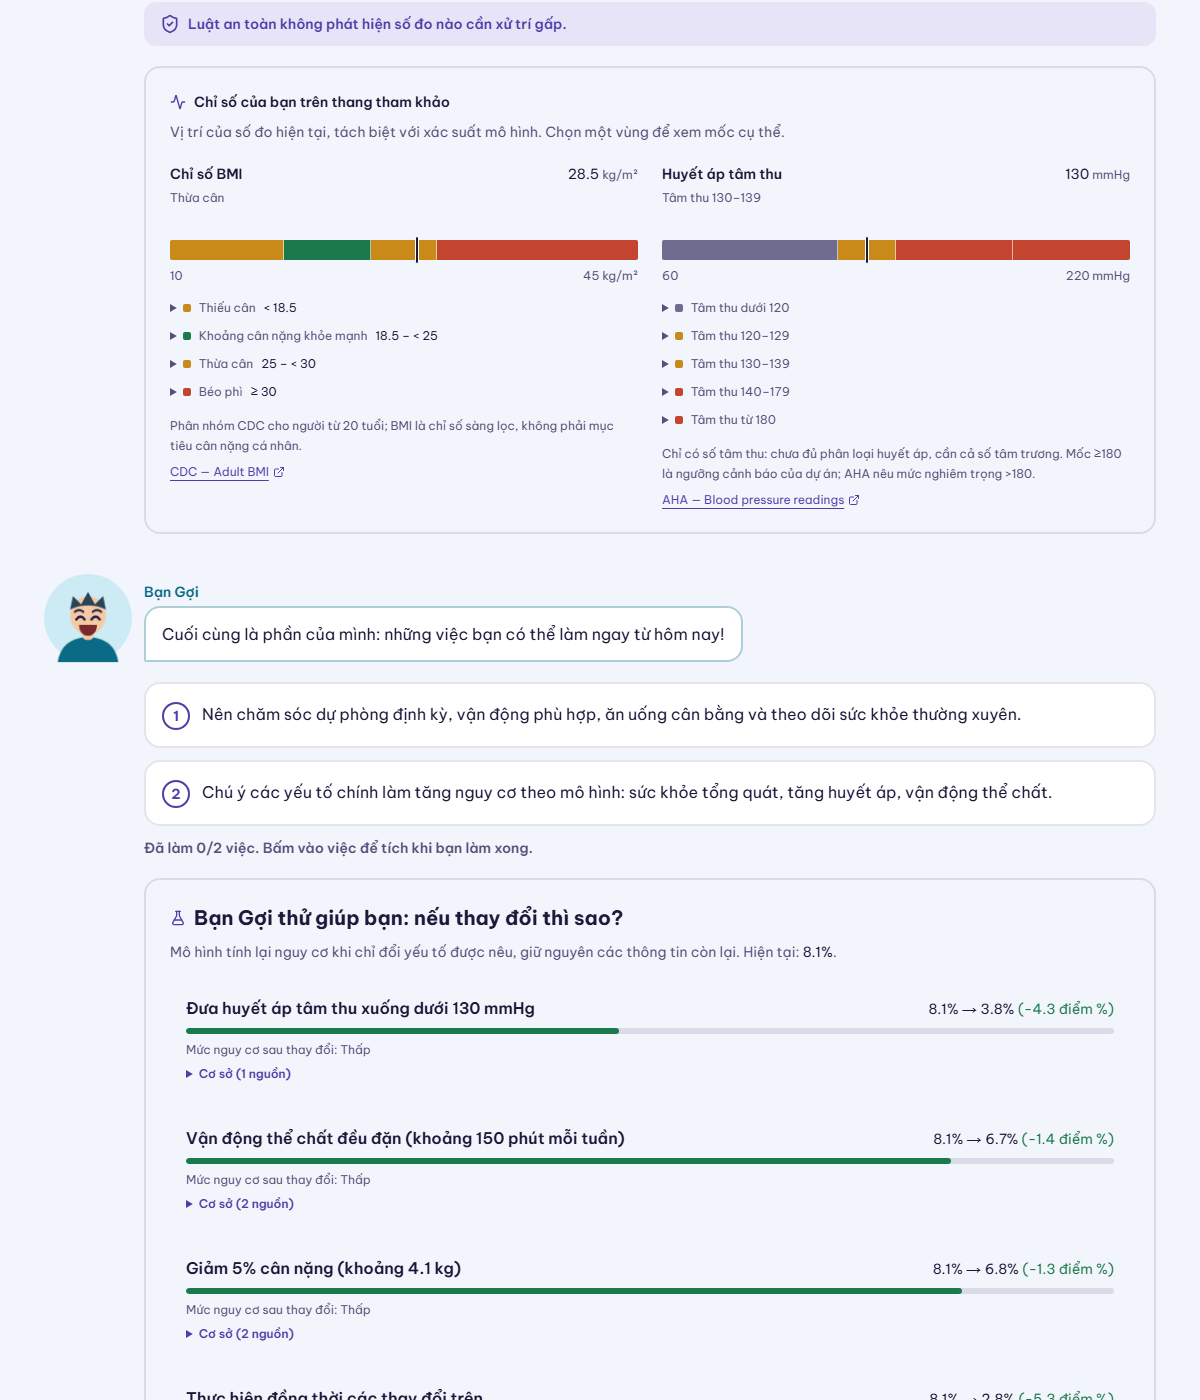
\includegraphics[width=0.92\textwidth]{images/ui_2c.png}
\caption{Cô Chứng trích dẫn bằng chứng; Chú Luật kiểm tra an toàn}\label{fig:ui2c}
\end{figure}
\begin{figure}[H]
\centering
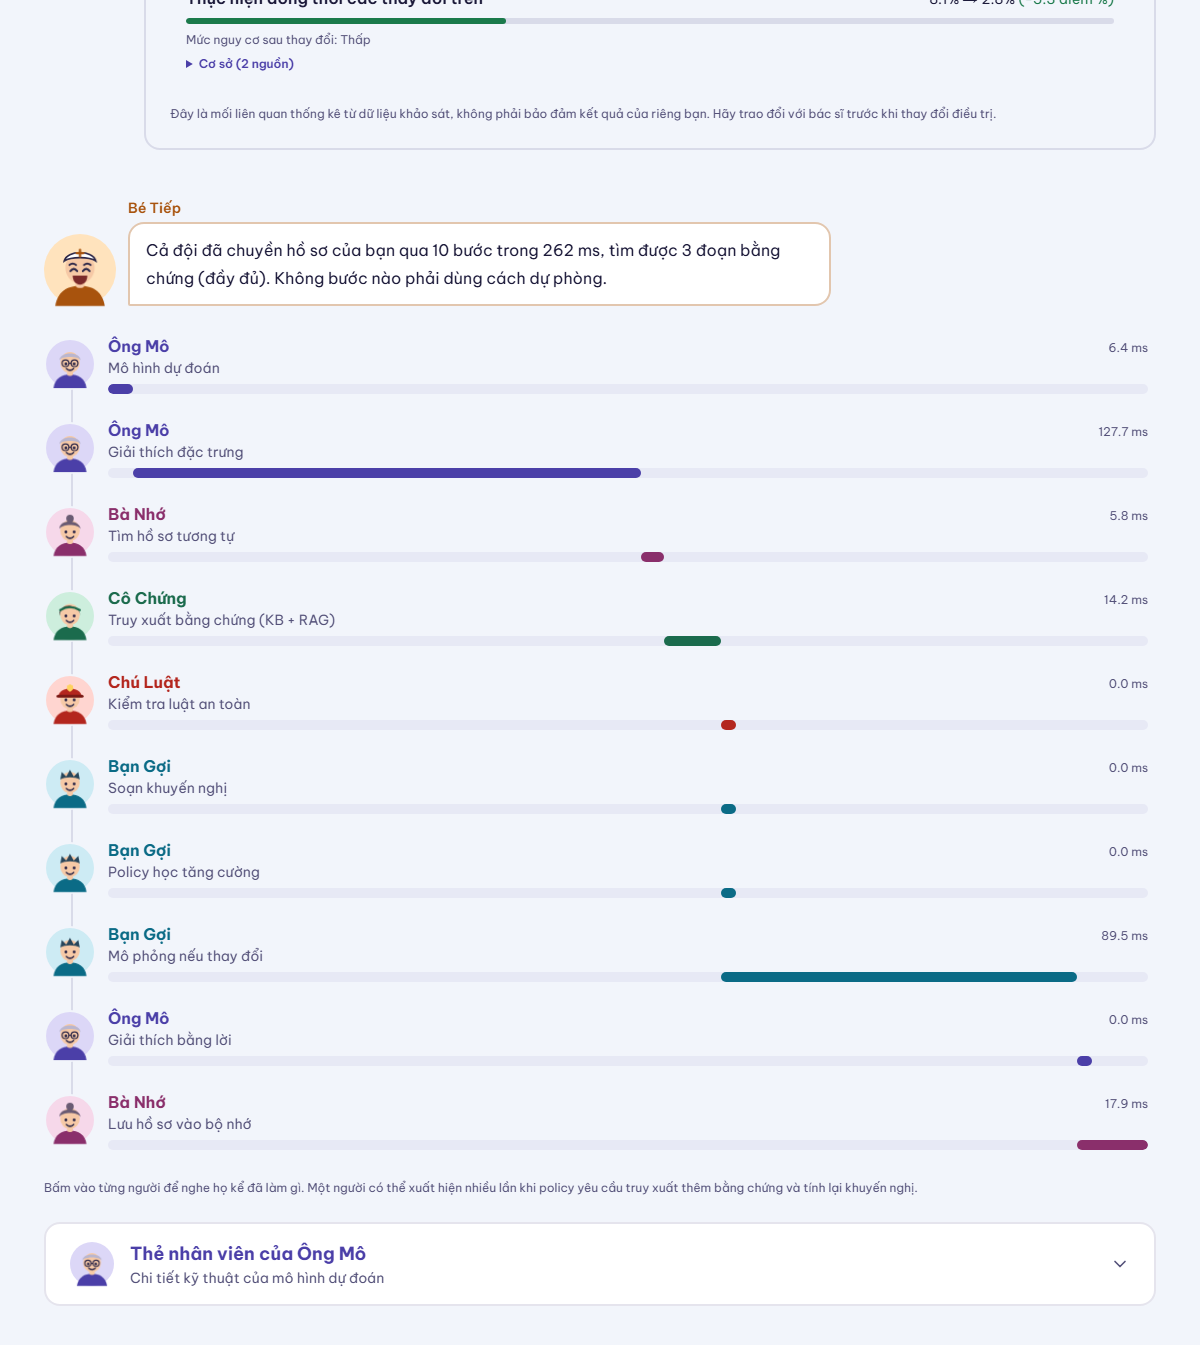
\includegraphics[width=0.92\textwidth]{images/ui_2d.png}
\caption{Thang chỉ số tham khảo, khuyến nghị của Bạn Gợi và \emph{trace} của lượt xử lý}\label{fig:ui2d}
\end{figure}

\section{Ví dụ ba lượt đánh giá}
Ba hồ sơ dưới đây được chạy thật qua \code{POST /v1/predict} (không LLM, \textbf{KB đọc từ tệp JSON vì lần chạy này không bật Neo4j}). Cột cuối cho thấy hành vi của hệ thống, không phải đánh giá lâm sàng.

\begin{table}[H]
\centering
\caption{Ba hồ sơ chạy thật qua API}\label{tab:cases}
\begin{tabularx}{\textwidth}{@{}L{2.6cm}L{3.2cm}L{3.2cm}X@{}}
\toprule
\textbf{} & \textbf{A: nam 58 tuổi, 170 cm, 90 kg, HA 150, glucose lúc đói 92} & \textbf{B: nữ 45 tuổi, 160 cm, 55 kg, HA 118, chưa đo glucose} & \textbf{C: 50 tuổi, 172 cm, 80 kg, HA 185, glucose 320}\\
\midrule
Xác suất MLP / mức & 17,3\% / Thấp & 0,5\% / Thấp & 3,9\% / Thấp\\
Luật kích hoạt & Không & Không & \code{GLU-300}, \code{BP-180}\\
Xung đột & Không & Không & \code{CF-PRED-LOW-MEASURED-HIGH}\\
\code{effective_risk} & Thấp & Thấp & \textbf{Cao}\\
Hướng xử trí & Theo dõi định kỳ & Theo dõi định kỳ & \textbf{Khám khẩn cấp}\\
Bằng chứng & 3 đoạn (đầy đủ) & 3 đoạn (đầy đủ) & 3 đoạn (đầy đủ)\\
Bước policy & \code{recommend_routine} & \code{request_glucose} & \code{escalate_to_clinician}\\
Câu hỏi bổ sung & Hỏi tiền sử đột quỵ & Hỏi kết quả glucose & Không (ưu tiên chuyển tuyến)\\
\emph{What-if} & 2 kịch bản & 0 & Không áp dụng\\
Tổng thời gian & 352 ms & 279 ms & 142 ms\\
\bottomrule
\end{tabularx}
\end{table}

Hồ sơ C minh họa nguyên tắc quan trọng nhất: mô hình chỉ thấy các yếu tố lối sống và cho xác suất 3,9\% (Thấp), nhưng huyết áp 185 mmHg và glucose 320 mg/dL kích hoạt hai luật khẩn cấp, luật xung đột \code{CF-PRED-LOW-MEASURED-HIGH} nâng \code{effective_risk} lên Cao, và policy không được phép hạ mức chuyển tuyến. Lượt chạy này cũng sinh một cuộc trao đổi hai thông điệp trong \code{trace.dialogue}: \code{SafetyGuard} $\rightarrow$ \code{RiskModel}, \code{challenge} (``mô hình dự đoán nguy cơ thấp nhưng số đo nằm trong khoảng nguy hiểm; ưu tiên số đo thực tế hơn dự đoán''), và \code{RiskModel} $\rightarrow$ \code{SafetyGuard}, \code{accept} (chấp nhận nâng nguy cơ hiệu lực lên Cao); hồ sơ A và B không có bất đồng nên \code{dialogue} rỗng. Hồ sơ B cho thấy hệ thống không coi ``chưa đo glucose'' là dấu hiệu yên tâm mà hỏi bổ sung. Với hồ sơ A, ba đoạn bằng chứng truy xuất gồm hai đoạn ADA (tiến triển từ tiền ĐTĐ, tuổi bắt đầu sàng lọc) và một đoạn WHO, hai trong ba đoạn được đồ thị gắn với yếu tố nguy cơ của bệnh nhân (\code{graph+semantic}). Thời gian chủ yếu nằm ở giải thích độ nhạy (khoảng 110--130 ms) và mô phỏng \emph{what-if} (khoảng 120 ms); các bước còn lại dưới 50 ms.

\section{Kiểm thử}
Bộ kiểm thử gồm \textbf{154 kiểm thử}, đều đạt trong lần chạy cuối (3 cảnh báo deprecation của SciPy), độ phủ \textbf{84\%} (\code{pytest --cov=.}).

\begin{table}[H]
\centering
\caption{Bộ kiểm thử tự động}\label{tab:tests}
\begin{tabularx}{\textwidth}{@{}L{4.3cm}X@{}}
\toprule
\textbf{Tệp} & \textbf{Nội dung}\\
\midrule
\code{test_api.py} & Các endpoint, kiểm tra đầu vào (thiếu BMI hoặc chiều cao/cân nặng trả 422), luồng trả lời câu hỏi bổ sung\\
\code{test_orchestrator.py} & Truyền kết quả giữa thành phần, cô lập lỗi, \code{degraded}\\
\code{test_rules.py} & Từng luật cơ sở và luật xung đột, quyền ưu tiên của số đo\\
\code{test_input_quality.py} & Lý do trừ điểm chất lượng dữ liệu khớp điểm số\\
\code{test_risk_model.py}, \code{test_risk_bands.py}, \code{test_mlp.py} & Ánh xạ huyết áp sang \code{HighBP}, mức nguy cơ theo artifact (cờ dương tính không bao giờ ở mức Thấp), MLP dự đoán được sau khi nạp mà không cần torch và hiệu chuẩn như các ứng viên khác\\
\code{test_retriever.py}, \code{test_neo4j_kb.py} & Truy xuất, trạng thái bằng chứng, nạp và truy vấn KB, dự phòng\\
\code{test_rl.py} & Môi trường, Q-learning, luật ghi đè policy\\
\code{test_dialogue.py} & Thông điệp giữa các thành phần: không bất đồng thì rỗng, \code{challenge} rồi \code{accept}/\code{propose}/\code{inform} đúng người nhận; đề xuất tìm mở rộng được thực hiện đúng một lần, đổi bằng chứng và khuyến nghị nhưng không hạ mức chuyển tuyến; tìm mở rộng lỗi thì giữ bằng chứng cũ và báo lỗi\\
\code{test_step11.py}, \code{test_patient_guidance.py}, \code{test_what_if.py}, \code{test_step12.py} & Giải thích không gán nhầm đặc trưng tự điền, điểm chất lượng theo tỉ lệ mục tự điền, hồ sơ tương tự theo khoảng cách số, thang chỉ số, câu hỏi bổ sung, mô phỏng \emph{what-if}, kịch bản chấp nhận trên artifact thật\\
\bottomrule
\end{tabularx}
\end{table}

\section{Đánh giá}
\textbf{Mô hình.} Xem Bảng~\ref{tab:models}: MLP hiệu chuẩn đạt ROC-AUC 0,826 và AP 0,414 trên 50.736 hồ sơ kiểm tra, ngang các mô hình boosting. Phân tầng có ý nghĩa: nhãn 1 chiếm 7,1\%, 32,1\% và 49,0\% lần lượt ở mức Thấp, Trung bình và Cao.

\textbf{Policy RL.} Xem Bảng~\ref{tab:rl}; chỉ có giá trị trong môi trường mô phỏng.

\textbf{Tích hợp.} Lần chạy demo tích hợp ngày 03/11/2026 (\code{scripts/demo_step12.py --require-neo4j --with-web}) đạt \textbf{26/26} kịch bản trên Neo4j thật (\code{kb_source = KnowledgeGraph}): hồ sơ đủ và thiếu dữ liệu, cảnh báo, thiếu bằng chứng, lỗi từng thành phần (retriever, memory, explainer, recommender, safety, policy), lỗi đầu vào (422), lịch sử, và cả ba proxy web khi backend ngừng (HTTP 502). Phần luồng hỏi bổ sung được kiểm tra bằng trình duyệt ở hai kích thước (1440$\times$1000 và 390$\times$844) với các kiểm tra như không hỏi lặp, không gán giá trị giả, không tràn bố cục. Lần chạy demo dùng mẫu câu dự phòng, chưa gọi OpenAI thật.

\textbf{Điều chưa được đánh giá.} Chưa có đánh giá đầu--cuối trên ca bệnh thật (độ nhạy/đặc hiệu của cả hệ thống), chưa có benchmark truy xuất, chưa có thử nghiệm người dùng, và các số đo độ trễ ở Bảng~\ref{tab:cases} chỉ là ba lần chạy, không phải thống kê.

\section{Hạn chế và hướng phát triển}
\begin{itemize}[nosep]
\item \textbf{Mô hình}: dữ liệu BRFSS 2015 chỉ của Hoa Kỳ, nhãn tự khai và gộp tiền ĐTĐ với ĐTĐ; chưa hiệu chỉnh cho người Việt; MLP không hơn rõ rệt các mô hình boosting. \code{HighBP} suy ra từ một số đo huyết áp là xấp xỉ.
\item \textbf{Glucose không vào mô hình}: xác suất MLP không đổi khi bổ sung glucose; glucose chỉ tác động qua luật và tư vấn.
\item \textbf{KB/RAG}: chỉ 21 đoạn bằng chứng từ 5 nguồn, chưa thẩm định chuyên môn; chưa có bộ đánh giá truy xuất; embedding MiniLM chủ yếu cho tiếng Anh. Hướng sửa: embedding đa ngôn ngữ, mở rộng KB, xây bộ câu hỏi có đáp án.
\item \textbf{Luật}: ngưỡng là của dự án, chưa được bác sĩ thẩm định.
\item \textbf{RL}: môi trường và phần thưởng tự đặt, chưa học từ phản hồi thật; không chứng minh hơn bảng kiểm cố định.
\item \textbf{Giao tiếp agent--agent còn tối thiểu}: các thành phần vẫn do Orchestrator gọi tuần tự. Phần phản biện (\code{challenge}/\code{accept}/\code{propose}/\code{inform}) dùng hàm phản hồi tất định; chỉ đề xuất tìm mở rộng bằng chứng của retriever được thực hiện thật, còn lại chỉ ghi lại bất đồng do luật xác định. Chưa có thương lượng nhiều vòng, chưa có agent nào tự khởi xướng hay thay đổi quyết định lâm sàng cuối, và đề xuất tìm mở rộng chưa kích hoạt trên hồ sơ thật vì bằng chứng của KB hiện tại luôn đủ. Lần chạy demo 26/26 thực hiện trước khi thêm phần này và chưa được chạy lại.
\item \textbf{Chưa có thử nghiệm với người dùng thật.} Mọi kết quả chỉ nhằm mục đích học tập, không thay thế tư vấn y khoa.
\end{itemize}

% ================= KẾT LUẬN =================
\chapter*{KẾT LUẬN}
\addcontentsline{toc}{chapter}{KẾT LUẬN}
Dự án đã hiện thực hóa sơ đồ hệ đa agent cho bệnh tiểu đường thành một hệ thống chạy được đầu--cuối. Dữ liệu BRFSS 2015 (253.680 hồ sơ) đi qua Deep Learning để dự đoán và phân loại nguy cơ: MLP PyTorch hiệu chuẩn đạt ROC-AUC 0,826 trên tập kiểm tra tách riêng, ngang các mô hình boosting, với ngưỡng và ba mức nguy cơ chọn trên tập kiểm định. Tri thức từ ADA, WHO, CDC, NIDDK và thử nghiệm DPP được tổ chức thành đồ thị Neo4j (20 thực thể, 35 quan hệ, 21 đoạn bằng chứng) và truy xuất bằng RAG kết hợp liên kết đồ thị, để khuyến nghị luôn kèm nguồn. Bộ luật 9 luật bảo đảm số đo thực tế thắng dự đoán thống kê, và policy Q-learning chọn bước tiếp theo luôn nằm dưới quyền ưu tiên của luật. Khi các thành phần bất đồng, chúng trao đổi thông điệp có kiểu (phản biện, chấp nhận, đề xuất, thông báo) được ghi vào \code{trace}. Hệ thống được kiểm thử bằng 154 kiểm thử tự động (độ phủ 84\%) và demo tích hợp 26/26 kịch bản trên Neo4j thật.

Bài học lớn nhất của dự án là trong bài toán y tế, giá trị của kiến trúc nhiều thành phần nằm ở chỗ mô hình thống kê, bằng chứng có nguồn và luật tường minh \emph{kiểm tra chéo} nhau, mọi kết quả truy vết được tới một bước cụ thể (\code{trace}), và phần học luôn đặt dưới sự giám sát của tri thức tường minh. Đồng thời, báo cáo nêu rõ các giới hạn: dữ liệu và nhãn của Hoa Kỳ, MLP không vượt trội, RL chỉ trên môi trường mô phỏng, chưa có benchmark truy xuất và chưa thẩm định chuyên môn. Hướng phát triển tiếp theo gồm: hiệu chỉnh mô hình trên dữ liệu người Việt, dùng embedding đa ngôn ngữ và xây bộ đánh giá truy xuất, nhờ chuyên gia y khoa thẩm định KB và ngưỡng luật, và mở rộng giao tiếp giữa các agent từ ghi nhận bất đồng sang thương lượng nhiều vòng.

% ================= TÀI LIỆU THAM KHẢO =================
\begin{thebibliography}{99}
\addcontentsline{toc}{chapter}{TÀI LIỆU THAM KHẢO}
\bibitem{ada2025} American Diabetes Association Professional Practice Committee, ``Standards of care in diabetes---2025,'' \emph{Diabetes Care}, vol. 48, no. Suppl. 1, 2025. \url{https://diabetesjournals.org/care/issue/48/Supplement_1}
\bibitem{dpp2002} Diabetes Prevention Program Research Group, ``Reduction in the incidence of type 2 diabetes with lifestyle intervention or metformin,'' \emph{New England Journal of Medicine}, vol. 346, no. 6, pp. 393--403, 2002.
\bibitem{who2024} World Health Organization, \emph{Diabetes fact sheet}, 2024. \url{https://www.who.int/news-room/fact-sheets/detail/diabetes}
\bibitem{cdc} Centers for Disease Control and Prevention, \emph{Diabetes risk factors and prevention}, 2024. \url{https://www.cdc.gov/diabetes/}
\bibitem{niddk} National Institute of Diabetes and Digestive and Kidney Diseases, \emph{Diabetes information}, 2024. \url{https://www.niddk.nih.gov/health-information/diabetes}
\bibitem{whelton2018} P. K. Whelton \emph{et al.}, ``2017 ACC/AHA guideline for the prevention, detection, evaluation, and management of high blood pressure in adults,'' \emph{Hypertension}, vol. 71, no. 6, pp. e13--e115, 2018.
\bibitem{uci891} Centers for Disease Control and Prevention, \emph{CDC Diabetes Health Indicators} (BRFSS 2015), UCI Machine Learning Repository, id 891. \url{https://archive.ics.uci.edu/dataset/891/cdc+diabetes+health+indicators}
\bibitem{wooldridge2009} M. Wooldridge, \emph{An Introduction to MultiAgent Systems}, 2nd ed. Wiley, 2009.
\bibitem{jennings1998} N. R. Jennings, K. Sycara, and M. Wooldridge, ``A roadmap of agent research and development,'' \emph{Autonomous Agents and Multi-Agent Systems}, vol. 1, pp. 7--38, 1998.
\bibitem{russell2021} S. Russell and P. Norvig, \emph{Artificial Intelligence: A Modern Approach}, 4th ed. Pearson, 2021.
\bibitem{fipa2002} Foundation for Intelligent Physical Agents, \emph{FIPA ACL message structure specification} (SC00061G), 2002.
\bibitem{lewis2020} P. Lewis \emph{et al.}, ``Retrieval-augmented generation for knowledge-intensive NLP tasks,'' in \emph{Advances in Neural Information Processing Systems (NeurIPS)}, 2020.
\bibitem{reimers2019} N. Reimers and I. Gurevych, ``Sentence-BERT: Sentence embeddings using Siamese BERT-networks,'' in \emph{EMNLP-IJCNLP}, 2019.
\bibitem{adamw} I. Loshchilov and F. Hutter, ``Decoupled weight decay regularization,'' in \emph{International Conference on Learning Representations (ICLR)}, 2019.
\bibitem{watkins1992} C. J. C. H. Watkins and P. Dayan, ``Q-learning,'' \emph{Machine Learning}, vol. 8, pp. 279--292, 1992.
\bibitem{sutton2018} R. S. Sutton and A. G. Barto, \emph{Reinforcement Learning: An Introduction}, 2nd ed. MIT Press, 2018.
\bibitem{neo4j} Neo4j, Inc., \emph{Neo4j graph database and the Cypher query language}. \url{https://neo4j.com/docs/}
\bibitem{chroma} Chroma, \emph{Chroma: the open-source embedding database}. \url{https://docs.trychroma.com/}
\end{thebibliography}

\end{document}
